%_____________________________________________________________________________
%=============================================================================
% main.tex v10 (02-10-2016) \ldots dibuat oleh Lionov - Informatika FTIS UNPAR 
% 
% Ini adalah file utama (main.tex), berisi perintah-perintah yang khusus 
% dibuat untuk template ini
%
% 			JANGAN MENGUBAH APAPUN DI DALAM FILE INI, 
%			KECUALI ANDA TAHU APA YANG ANDA LAKUKAN !!! 
% 
% Perubahan pada versi 10 (02-10-2016):
%	- Perubahan nama file dari main.tex menjadi skripsi.tex
%	- Perubahan style bibliography dari "ieeetr" menjadi "compj" yang digunakan
%     di jurnal "The Computer Journal" yg diterbitkan oleh Oxford University 
%     Press/British Computer Society
%	- Penempatan gambar otomatis di folder "Gambar", jadi tidak perlu menuliskan
%	  nama folder lagi (\includegraphics{Gambar/tes} --> \includegraphics{tes})
%	- Perubahan font menjadi latin modern yg sdh banyak digunakan di jurnal2 intl
%   - Perbaikan kecil: jeda antara ttd pembimbing dan penguji
%	- Pembimbing Tunggal --> Pembimbing (karena sdh jelas tunggal 
%	- Penggunaan kantlipsum (output bhs inggris) sebagai pengganti lipsum
%	- \onespacing otomatis untuk buku skripsi final, untuk buku sidang tetap 
%	  \onehalfspacing
%	- Perbaikan hfill dan hfil yang masih menjadi masalah, bagian itu dipindahkan
%	  ke dekat deklarasi Daftar Isi
%_____________________________________________________________________________
%=============================================================================

%setup.tex
\documentclass[11pt,a4paper,twoside,openright,notitlepage]{report}  

\usepackage{lmodern} %font latin modern 
\usepackage[bahasa]{babel} %bahasa indonesia
\usepackage[T1]{fontenc}  %encoding
% \usepackage{mathptmx}
% \usepackage{venturisold}
% \usepackage{helvet}
% \usepackage{fouriernc} 
\usepackage{abstract} %manipulasi abstract
\usepackage{chappg} % format daftar isi 
\usepackage{color} %warna 
\usepackage{etoolbox} %untuk programming if-then
\usepackage{fancyhdr} %format header & footer
\usepackage{float} %penempatan gambar di tempat yg seharusnya 
\usepackage[inner=2.5cm,outer=2cm,top=2.5cm,bottom=2.5cm]{geometry} %margin
\usepackage{graphicx} %gambar
\usepackage{listings} %source code
\usepackage{lscape} %landscape untuk source code
\usepackage{multicol} %multiple column
\usepackage{ifthen} % if then
\usepackage[pagewise]{lineno} %line numbering
\usepackage{kantlipsum} % untuk dummy text
\usepackage{titlesec} %judul header
\usepackage{tocbibind} %daftar isi, gambar, tabel dll
\usepackage{tocloft} % format daftar isi 
\usepackage{setspace} %line spacing
\usepackage{xstring} %manipulasi string
\usepackage[plainpages=false,pdfpagelabels,unicode]{hyperref} %\autoref, \phantomsection & link 
\usepackage{emptypage} %halaman kosong antar bab

\usepackage{rotating}
\usepackage{pdflscape}
\usepackage{adjustbox}
%\usepackage{blindtext}


\graphicspath{{./Gambar/}} 

\usepackage{lcg}
\newcommand{\random}{\rand\arabic{rand}}

\let\abstractname\Abstrak

\normalfont
\DeclareFontShape{T1}{lmr}{bx}{sc} { <-> ssub * cmr/bx/sc }{}

\titleformat{\chapter}[display] {\Large\bfseries\centering}{\MakeUppercase{\chaptertitlename} \thechapter}{15pt}{\Large\MakeUppercase}

\renewcommand{\cftchapfont}{\scshape \bfseries}

% Tidak perlu ada kata "Bab", "Gambar" atau "Tabel" di daftar 
% \renewcommand{\cftchappresnum}{{\bf \scshape Bab} } 
% \renewcommand{\cftchapnumwidth}{1.5cm}
% \renewcommand{\cftfigpresnum}{{Gambar\ }} 
% \renewcommand{\cftfignumwidth}{2.5cm}
% \renewcommand{\cfttabpresnum}{{Tabel\ }} 
% \renewcommand{\cfttabnumwidth}{2cm}


\newcommand{\vnama}{Jane Doe}
\newcommand{\vlnama}{John Doe}
\newcommand{\vnpm}{1992700001}
\newcommand{\vprodiINA}{SAINS}
\newcommand{\vprodiENG}{SCIENCE}
\newcommand{\vstaINA}{UJIAN}
\newcommand{\vstaENG}{EXAM}
%\newcommand{\vjudul}{Judul Skripsi/Tugas Akhir}
\newcommand{\vpembu}{Plato}
\newcommand{\vpembs}{Euclid}
\newcommand{\vpengi}{Plato}
\newcommand{\vpengii}{Euclid}
\newcommand{\vtanggal}{1}
\newcommand{\vbulan}{Januari}
\newcommand{\vtahun}{1970}
\newcommand{\vmode}{final}
\newcommand{\vspacing}{double}
\newcommand{\vlineno}{yes}
\newcommand{\vkunciina}{Skripsi, Tugas Akhir}
\newcommand{\vkuncieng}{Undergraduate Thesis, Final Project}
\newcommand{\vkajur}{Jack Doe}
\newcommand{\vkajurmat}{Jack Doe}
\newcommand{\vkajurfis}{Jack Doe}
\newcommand{\vkajurtif}{Jack Doe}
\newcommand{\vtabel}{}
\newcommand{\vgambar}{}
\newcommand{\vdierror}{}

\newcommand{\namanpm}[2]{
	\renewcommand{\vstaINA}{<<SKRIPSI/TUGAS AKHIR>>}
	\renewcommand{\vprodiINA}{<<MATEMATIKA/FISIKA/TEKNIK INFORMATIKA>>}
	\renewcommand{\vstaENG}{<<FINAL PROJECT/UNDERGRADUATE THESIS>>}
	\renewcommand{\vprodiENG}{<<MATHEMATICS/PHYSICS/INFORMATICS>>}
	\renewcommand{\vnama}{\uppercase{#1}} \renewcommand{\vlnama}{#1} \hypersetup{pdfauthor={#2 - #1}}
	\renewcommand{\vnpm}{#2} \hypersetup{pdfcreator={#2}} \StrChar{\vnpm}{6}[\vprodiN]
%	\renewcommand{\vnpm}{#2} \hypersetup{pdfcreator={\jobname}} \StrChar{\vnpm}{6}[\vprodiN]
	\ifdefstring{\vprodiN}{1}{
		\renewcommand{\vprodiINA}{MATEMATIKA} \renewcommand{\vprodiENG}{MATHEMATICS} 
		\renewcommand{\vstaINA}{SKRIPSI} \renewcommand{\vstaENG}{FINAL PROJECT} \renewcommand{\vkajur}{\vkajurmat}}{}
	\ifdefstring{\vprodiN}{2}{
		\renewcommand{\vprodiINA}{FISIKA} \renewcommand{\vprodiENG}{PHYSICS} 
		\renewcommand{\vstaINA}{TUGAS AKHIR} \renewcommand{\vstaENG}{FINAL PROJECT} \renewcommand{\vkajur}{\vkajurfis}}{}
	\ifdefstring{\vprodiN}{3}{
		\renewcommand{\vprodiINA}{TEKNIK INFORMATIKA} \renewcommand{\vprodiENG}{INFORMATICS} 
		\renewcommand{\vstaINA}{SKRIPSI} \renewcommand{\vstaENG}{UNDERGRADUATE THESIS} \renewcommand{\vkajur}{\vkajurtif}}{}
	}

%\newcommand{\judul}[1]{\renewcommand{\vjudul}{\uppercase{#1}}\hypersetup{pdftitle={#1}, pdfsubject={#1}}}
\newcommand{\pembimbing}[2]{\renewcommand{\vpembu}{#1}\renewcommand{\vpembs}{#2}}
\newcommand{\penguji}[2]{\renewcommand{\vpengi}{#1}\renewcommand{\vpengii}{#2}}
\newcommand{\kajur}[3]{\renewcommand{\vkajurmat}{#1}\renewcommand{\vkajurfis}{#2}\renewcommand{\vkajurtif}{#3}}
\renewcommand{\vbulan}{<<bulan>>}
\newcommand{\tanggal}[3]{\renewcommand{\vtanggal}{#1}\renewcommand{\vtahun}{#3}
	\newcommand{\vcbulan}{#2}
	\ifdefstring{\vcbulan}{1}{\renewcommand{\vbulan}{Januari}}{}
	\ifdefstring{\vcbulan}{2}{\renewcommand{\vbulan}{Februari}}{}
	\ifdefstring{\vcbulan}{3}{\renewcommand{\vbulan}{Maret}}{}
	\ifdefstring{\vcbulan}{4}{\renewcommand{\vbulan}{April}}{}
	\ifdefstring{\vcbulan}{5}{\renewcommand{\vbulan}{Mei}}{}
	\ifdefstring{\vcbulan}{6}{\renewcommand{\vbulan}{Juni}}{}
	\ifdefstring{\vcbulan}{7}{\renewcommand{\vbulan}{Juli}}{}
	\ifdefstring{\vcbulan}{8}{\renewcommand{\vbulan}{Agustus}}{}
	\ifdefstring{\vcbulan}{9}{\renewcommand{\vbulan}{September}}{}
	\ifdefstring{\vcbulan}{10}{\renewcommand{\vbulan}{Oktober}}{}
	\ifdefstring{\vcbulan}{11}{\renewcommand{\vbulan}{November}}{}
	\ifdefstring{\vcbulan}{12}{\renewcommand{\vbulan}{Desember}}{}	
}

\newcommand{\judulINA}[1]{\newcommand{\vjudulINA}{\uppercase{#1}}\hypersetup{pdftitle={#1},pdfsubject={#1}}}
\newcommand{\judulENG}[1]{\newcommand{\vjudulENG}{\uppercase{#1}}\hypersetup{pdftitle={#1},pdfsubject={#1}}}
\newcommand{\abstrakINA}[1]{\newcommand{\vabstrakina}{#1}}
\newcommand{\abstrakENG}[1]{\newcommand{\vabstrakeng}{#1}}
\newcommand{\kunciINA}[1]{\renewcommand{\vkunciina}{#1} \hypersetup{pdfkeywords={#1}}}
\newcommand{\kunciENG}[1]{\renewcommand{\vkuncieng}{#1}}
\newcommand{\untuk}[1]{\newcommand{\vuntuk}{#1}}
\newcommand{\prakata}[1]{\newcommand{\vprakata}{#1}}
\newcommand{\mode}[1]{\renewcommand{\vmode}{#1}}
\newcommand{\linespacing}[1]{\renewcommand{\vspacing}{#1}}
\newcommand{\linenumber}[1]{\renewcommand{\vlineno}{#1}}

\newcommand{\daftarIsiError}[1]{\renewcommand{\vdierror}{#1}} 
\newcommand{\gambar}[1]{\renewcommand{\vgambar}{#1}}
\newcommand{\tabel}[1]{\renewcommand{\vtabel}{#1}}

\newcommand{\bab}[1]{\newcommand{\vbab}{#1}}
\newcommand{\lampiran}[1]{\renewcommand{\vlmp}{#1}} 

\newcommand{\vpilbab}{0}
\newcommand{\vbaba}{0}\newcommand{\vbabb}{0}\newcommand{\vbabc}{0}
\newcommand{\vbabd}{0}\newcommand{\vbabe}{0}\newcommand{\vbabf}{0}
\newcommand{\vbabg}{0}\newcommand{\vbabh}{0}\newcommand{\vbabi}{0}
\newcommand{\vpillmp}{0}
\newcommand{\vlmpa}{0}\newcommand{\vlmpb}{0}\newcommand{\vlmpc}{0}
\newcommand{\vlmpd}{0}\newcommand{\vlmpe}{0}\newcommand{\vlmpf}{0}
\newcommand{\vlmpg}{0}\newcommand{\vlmph}{0}\newcommand{\vlmpi}{0}
\newcommand{\vlmp}{x}

%	\ifdefempty{#1}{\bab{1,2,3,4,5,6,7,8,9} \tampilbab{\vbab}}{
\newcommand{\tampilbab}[1]{
	\ifdefempty{#1}{
		\renewcommand{\vbaba}{1}\renewcommand{\vbabb}{1}\renewcommand{\vbabc}{1}
		\renewcommand{\vbabd}{1}\renewcommand{\vbabe}{1}\renewcommand{\vbabf}{1}
		\renewcommand{\vbabg}{1}\renewcommand{\vbabh}{1}\renewcommand{\vbabi}{1}}{
	\renewcommand{\do}[1]{
		\renewcommand{\vpilbab}{##1}
		\ifdefstring{\vpilbab}{1}{\renewcommand{\vbaba}{1}}{}
		\ifdefstring{\vpilbab}{2}{\renewcommand{\vbabb}{1}}{}
		\ifdefstring{\vpilbab}{3}{\renewcommand{\vbabc}{1}}{}
		\ifdefstring{\vpilbab}{4}{\renewcommand{\vbabd}{1}}{}
		\ifdefstring{\vpilbab}{5}{\renewcommand{\vbabe}{1}}{}
		\ifdefstring{\vpilbab}{6}{\renewcommand{\vbabf}{1}}{}
		\ifdefstring{\vpilbab}{7}{\renewcommand{\vbabg}{1}}{}
		\ifdefstring{\vpilbab}{8}{\renewcommand{\vbabh}{1}}{}
		\ifdefstring{\vpilbab}{9}{\renewcommand{\vbabi}{1}}{}
	}
	\expandafter\docsvlist\expandafter{#1}
	}
}

\newcommand{\tampillmp}[1]{
	\ifdefempty{#1}{
		\renewcommand{\vlmpa}{1}\renewcommand{\vlmpb}{1}\renewcommand{\vlmpc}{1}
		\renewcommand{\vlmpd}{1}\renewcommand{\vlmpe}{1}\renewcommand{\vlmpf}{1}
		\renewcommand{\vlmpg}{1}\renewcommand{\vlmph}{1}\renewcommand{\vlmpi}{1}}{
	\ifdefstring{#1}{-1}{ }{
		\renewcommand{\do}[1]{ 
			\renewcommand{\vpillmp}{##1}
			\ifdefstring{\vpillmp}{A}{\renewcommand{\vlmpa}{1}}{}
			\ifdefstring{\vpillmp}{B}{\renewcommand{\vlmpb}{1}}{}
			\ifdefstring{\vpillmp}{C}{\renewcommand{\vlmpc}{1}}{}
			\ifdefstring{\vpillmp}{D}{\renewcommand{\vlmpd}{1}}{}
			\ifdefstring{\vpillmp}{E}{\renewcommand{\vlmpe}{1}}{}
			\ifdefstring{\vpillmp}{F}{\renewcommand{\vlmpf}{1}}{}
			\ifdefstring{\vpillmp}{G}{\renewcommand{\vlmpg}{1}}{}
			\ifdefstring{\vpillmp}{H}{\renewcommand{\vlmph}{1}}{}
			\ifdefstring{\vpillmp}{I}{\renewcommand{\vlmpi}{1}}{}}
		}
	\expandafter\docsvlist\expandafter{#1}
	}
}

\newcommand{\appspacing}{
	\ifdefstring{\vspacing}{single}{\singlespacing}{}
	\ifdefstring{\vspacing}{onehalf}{\onehalfspacing}{}
	\ifdefstring{\vspacing}{double}{\doublespacing}{}
	\ifdefstring{\vmode}{sidang}{\onehalfspacing}{}	
	\ifdefstring{\vmode}{sidang_akhir}{\onehalfspacing}{}	
	\ifdefstring{\vmode}{final}{\singlespacing}{}
}

\newcommand{\appline}{
	\ifdefstring{\vmode}{final}{\renewcommand{\vlineno}{no}}{}
	\ifdefstring{\vlineno}{yes}{\linenumbers \def\linenumberfont{\normalfont\tiny\sffamily}}{}
	\ifdefstring{\vlineno}{no}{\lstset{numbers=left, stepnumber=1, numbersep=5pt}}{}
	
}

\newcommand{\appmargin}{
	\ifdefstring{\vmode}{final}{}{\newgeometry{inner=3cm,outer=2.75cm,top=2cm,bottom=2cm}}
}

\renewcommand{\abstractnamefont}{\bf \MakeUppercase}

\makeatletter
\def\headrule{{%
  \if@fancyplain\let\headrulewidth\plainheadrulewidth\fi
  \hrule\@height\footrulewidth\@width\headwidth\vskip2pt%
  \hrule\@height\headrulewidth\@width\headwidth\vskip-\headrulewidth\vskip-4pt
}}
\def\footrule{}

\def\cleardoublepage{
	\clearpage
	\if@twoside \ifodd\c@page
	\else
		\hbox{}
		\vspace{\fill} 
		\thispagestyle{empty}
		\newpage
	\if@twocolumn\hbox{}\newpage\fi\fi\fi}
\makeatother

\renewcommand{\headrulewidth}{1.25pt}
\renewcommand{\footrulewidth}{0.25pt}

\setlength{\headheight}{15pt}
\fancyhead[LE,RO]{\thepage}
\fancyhead[RE]{\small{\textsc{\nouppercase{\leftmark}}}}
\fancyhead[LO]{\small{\textsc{\nouppercase{\rightmark}}}}
\fancyfoot{}

\hypersetup{unicode=true,colorlinks=true,linkcolor=blue,citecolor=green,filecolor=magenta, urlcolor=cyan}

\lstset{basicstyle=\tiny, commentstyle=\color{blue}}
\lstset{frame=leftline, tabsize=4, breaklines=true}

%end setup.tex

%_____________________________________________________________________________
%=============================================================================
% data.tex v8 (02-10-2016) \ldots dibuat oleh Lionov - Informatika FTIS UNPAR
%
% Perubahan pada versi 8 (02-10-2016)
%	- Perubahan keterangan pada spacing: Otomatis spasi 1 untuk buku skripsi 
%	  final dan 1.5 untuk buku sidang
%	- Penggunaan kantlipsum
%_____________________________________________________________________________
%=============================================================================

%=============================================================================
% 								PETUNJUK
%=============================================================================
% Ini adalah file data (data.tex)
% Masukkan ke dalam file ini, data-data yang diperlukan oleh template ini
% Cara memasukkan data dijelaskan di setiap bagian
% Data yang WAJIB dan HARUS diisi dengan baik dan benar adalah SELURUHNYA !!
% Hilangkan tanda << dan >> jika anda menemukannya
%=============================================================================

%_____________________________________________________________________________
%=============================================================================
% 								BAGIAN 0
%=============================================================================
% PERHATIAN!! PERHATIAN!! Bagian ini hanya ada untuk sementara saja
% Jika "DAFTAR ISI" tidak bisa berada di bagian tengah halaman, isi dengan XXX
% jika sudah benar posisinya, biarkan kosong (i.e. \daftarIsiError{ })
%=============================================================================
\daftarIsiError{ }
%=============================================================================

%_____________________________________________________________________________
%=============================================================================
% 								BAGIAN I
%=============================================================================
% Tambahkan package2 lain yang anda butuhkan di sini
%=============================================================================
\usepackage{booktabs} 
\usepackage[table]{xcolor}
\usepackage{longtable}
\usepackage{amssymb}
\usepackage{todo}
\usepackage{verbatim} 		%multilne comment
\usepackage{pgfplots}
%=============================================================================

%_____________________________________________________________________________
%=============================================================================
% 								BAGIAN II
%=============================================================================
% Mode dokumen: menetukan halaman depan dari dokumen, apakah harus mengandung 
% prakata/pernyataan/abstrak dll (termasuk daftar gambar/tabel/isi) ?
% - kosong : tidak ada halaman depan sama sekali (untuk dokumen yang 
%            dipergunakan pada proses bimbingan)
% - cover : cover saja tanpa daftar isi, gambar dan tabel
% - sidang : cover, daftar isi, gambar, tabel 
% - sidang_akhir : mode sidang + abstrak + abstract
% - final : seluruh halaman awal dokumen (untuk cetak final)
% Jika tidak ingin mencetak daftar tabel/gambar (misalkan karena tidak ada 
% isinya), edit manual di baris 439 dan 440 pada file main.tex
%=============================================================================
% \mode{kosong}
% \mode{cover}
% \mode{sidang}
% \mode{sidang_akhir}
\mode{sidang_akhir} 
%=============================================================================

%_____________________________________________________________________________
%=============================================================================
% 								BAGIAN III
%=============================================================================
% Line numbering: penomoran setiap baris, otomatis di-reset setiap berganti
% halaman
% - yes: setiap baris diberi nomor
% - no : baris tidak diberi nomor, otomatis untuk mode final
%=============================================================================
\linenumber{no}
%=============================================================================

%_____________________________________________________________________________
%=============================================================================
% 								BAGIAN IV
%=============================================================================
% Linespacing: jarak antara baris 
% - single	: wajib (dan otomatis jika ingin mencetak buku skripsi, opsi yang 
%			  disediakan untuk bimbingan, jika pembimbing tidak keberatan 
%			  (untuk menghemat kertas)
% - onehalf	: default dan wajib (dan otomatis) jika ingin mencetak dokumen
%             untuk sidang.
% - double 	: jarak yang lebih lebar lagi, jika pembimbing berniat memberi 
%             catatan yg banyak di antara baris (dianjurkan untuk bimbingan)
%=============================================================================
\linespacing{single}
%\linespacing{onehalf}
%\linespacing{double}
%=============================================================================

%_____________________________________________________________________________
%=============================================================================
% 								BAGIAN V
%=============================================================================
% Tidak semua skripsi memuat gambar dan/atau tabel. Untuk skripsi yang seperti
% itu, tidak diperlukan Daftar Gambar dan Daftar Tabel. Sayangnya hal ini 
% sulit dilakukan secara manual karena membutuhkan kedisiplinan pengguna 
% template.  
% Jika tidak akan menampilkan Daftar Gambar/Tabel, isi dengan NO. Jika ingin
% menampilkan, kosongkan parameter (i.e. \gambar{ }, \tabel{ })
%=============================================================================
\gambar{ }
\tabel{ }
%=============================================================================

%_____________________________________________________________________________
%=============================================================================
% 								BAGIAN VI
%=============================================================================
% Bab yang akan dicetak: isi dengan angka 1,2,3 s.d 9, sehingga bisa digunakan
% untuk mencetak hanya 1 atau beberapa bab saja
% Jika lebih dari 1 bab, pisahkan dengan ',', bab akan dicetak terurut sesuai 
% urutan bab (e.g. \bab{1,2,3}).
% Untuk mencetak seluruh bab, kosongkan parameter (i.e. \bab{ })  
% Catatan: Jika ingin menambahkan bab ke-10 dan seterusnya, harus dilakukan 
% secara manual
%=============================================================================
\bab{ }
%=============================================================================

%_____________________________________________________________________________
%=============================================================================
% 								BAGIAN VII
%=============================================================================
% Lampiran yang akan dicetak: isi dengan huruf A,B,C s.d I, sehingga bisa 
% digunakan untuk mencetak hanya 1 atau beberapa lampiran saja
% Jika lebih dari 1 lampiran, pisahkan dengan ',', lampiran akan dicetak 
% terurut sesuai urutan lampiran (e.g. \bab{A,B,C}).
% Jika tidak ingin mencetak lampiran apapun, isi dengan -1 (i.e. \lampiran{-1})
% Untuk mencetak seluruh mapiran, kosongkan parameter (i.e. \lampiran{ })  
% Catatan: Jika ingin menambahkan lampiran ke-J dan seterusnya, harus 
% dilakukan secara manual
%=============================================================================
\lampiran{ }
%=============================================================================

%_____________________________________________________________________________
%=============================================================================
% 								BAGIAN VIII
%=============================================================================
% Data diri dan skripsi/tugas akhir
% - namanpm: Nama dan NPM anda, penggunaan huruf besar untuk nama harus benar
%			 dan gunakan 10 digit npm UNPAR, PASTIKAN BAHWA BENAR !!!
%			 (e.g. \namanpm{Jane Doe}{1992710001}
% - judul : Dalam bahasa Indonesia, perhatikan penggunaan huruf besar, judul
%			tidak menggunakan huruf besar seluruhnya !!! 
% - tanggal : isi dengan {tangga}{bulan}{tahun} dalam angka numerik, jangan 
%			  menuliskan kata (e.g. AGUSTUS) dalam isian bulan
%			  Tanggal ini adalah tanggal dimana anda akan melaksanakan sidang 
%			  ujian akhir skripsi/tugas akhir
% - pembimbing: isi dengan pembimbing anda, lihat daftar dosen di file dosen.tex
%				jika pembimbing hanya 1, kosongkan parameter kedua 
%				(e.g. \pembimbing{\JND}{  } ) , \JND adalah kode dosen
% - penguji : isi dengan para penguji anda, lihat daftar dosen di file dosen.tex
%				(e.g. \penguji{\JHD}{\JCD} ) , \JND dan \JCD adalah kode dosen
% !!Lihat singkatan pembimbing dan penguji anda di file dosen.tex
%=============================================================================
\namanpm{Lucky Senjaya Darmawan}{2012730009}	%hilangkan tanda << & >>
\tanggal{}{05}{2017}			%hilangkan tanda << & >>
\pembimbing{GDK}{<<pembimbing pendamping/2>>} %hilangkan tanda << & >>    
\penguji{<<penguji 1>>}{<<penguji 2>>} 				%hilangkan tanda << & >>
%=============================================================================

%_____________________________________________________________________________
%=============================================================================
% 								BAGIAN IX
%=============================================================================
% Judul dan title : judul bhs indonesia dan inggris
% - judulINA: judul dalam bahasa indonesia
% - judulENG: title in english
% PERHATIAN: - langsung mulai setelah '{' awal, jangan mulai menulis di baris 
%			   bawahnya
%			 - Gunakan \texorpdfstring{\\}{} untuk pindah ke baris baru
%			 - Judul TIDAK ditulis dengan menggunakan huruf besar seluruhnya !!
%			 - Gunakan perintah \texorpdfstring{\\}{} untuk baris baru
%=============================================================================
\judulINA{Studi dan Integrasi \textit{Workflow} menggunakan BPMS dan Sistem Email}
\judulENG{Study and Workflow Integration using BPMS and Email System}
%_____________________________________________________________________________
%=============================================================================
% 								BAGIAN X
%=============================================================================
% Abstrak dan abstract : abstrak bhs indonesia dan inggris
% - abstrakINA: abstrak bahasa indonesia
% - abstrakENG: abstract in english
% PERHATIAN: langsung mulai setelah '{' awal, jangan mulai menulis di baris 
%			 bawahnya
%=============================================================================
\abstrakINA{\textit{Workflow} merupakan pemodelan proses bisnis yang dapat digambarkan sebagai \textit{flow map} atau BPMN \textit{(Business Process Model and Notation).} \textit{Workflow} ini dapat diotomasi menggunakan BPMS \textit{(Business Process Management System)}, seperti Camunda. Agar eksekusi \textit{workflow} lebih alamiah dengan model komunikasi organisasi saat ini, maka \textit{event} dapat dipropagasi dan diintegrasikan dengan sistem email. 

Dalam skripsi ini, akan dibuat suatu integrasi antara \textit{user task} dan sistem email. \textit{User task} adalah suatu tugas yang perlu dilakukan oleh pengguna. Ketika ada suatu \textit{user task}, sistem email akan mengirimkan email ke pengguna yang akan mengerjakan task tersebut. Email tersebut berisi tautan yang mengarah ke tugas yang perlu dikerjakan tersebut.}

\abstrakENG{Workflow is business process model that can be described as a flow map or BPMN (Business Process Model and Notation). Workflow can be automated using BPMS (Business Process Management System), such as Camunda. Workflow execution will be more natural with current orgaizational communication models, event can be propagated and integrated with email system.

This thesis will develop integration between user task and email system. User task is task that need to be done by the user. When there is a user task, email system will send email to user. The email contains link to the task that needs to be done.} 
%=============================================================================

%_____________________________________________________________________________
%=============================================================================
% 								BAGIAN XI
%=============================================================================
% Kata-kata kunci dan keywords : diletakkan di bawah abstrak (ina dan eng)
% - kunciINA: kata-kata kunci dalam bahasa indonesia
% - kunciENG: keywords in english
%=============================================================================
\kunciINA{Alur Kerja, Proses Bisnis, BPMN, BPMS, Camunda, Email}
\kunciENG{Workflow, Business Process, BPMN, BPMS, Camunda, Email}
%=============================================================================

%_____________________________________________________________________________
%=============================================================================
% 								BAGIAN XII
%=============================================================================
% Persembahan : kepada siapa anda mempersembahkan skripsi ini ...
%=============================================================================
\untuk{<<kepada siapa anda mempersembahkan skripsi ini\ldots?>>}
%=============================================================================

%_____________________________________________________________________________
%=============================================================================
% 								BAGIAN XIII
%=============================================================================
% Kata Pengantar: tempat anda menuliskan kata pengantar dan ucapan terima 
% kasih kepada yang telah membantu anda bla bla bla ....  
%=============================================================================
\prakata{\kant[3-4]}
%=============================================================================

%_____________________________________________________________________________
%=============================================================================
% 								BAGIAN XIV
%=============================================================================
% Tambahkan hyphen (pemenggalan kata) yang anda butuhkan di sini 
%=============================================================================
\hyphenation{ma-te-ma-ti-ka}
\hyphenation{fi-si-ka}
\hyphenation{tek-nik}
\hyphenation{in-for-ma-ti-ka}
%=============================================================================

%_____________________________________________________________________________
%=============================================================================
% 								BAGIAN XV
%=============================================================================
% Tambahkan perintah yang anda buat sendiri di sini 
%=============================================================================
\newcommand{\vtemplateauthor}{lionov}
\pgfplotsset{compat=newest}
\usetikzlibrary{patterns}
%=============================================================================

% Copyright \textcopyright [Lionov] [09-10-2016]. All rights reserved
%_____________________________________________________________________________
%=============================================================================
% dosen.tex v6 (19-08-2016) \ldots dibuat oleh Lionov - Informatika FTIS UNPAR
%
% Perubahan pada versi 6 (19-08-2016)
% 	- Penambahan dosen (Farica, Claudio).
%	- Penghapusan dosen (Oerip)
% 	- Perubahan singkatan untuk dosen Informatika sesuai ketentuan prodi
%	- Perbaikan "catatan untuk mhs teknik informatika"
%
% Perubahan pada versi sebelumnya dapat dilihat di bagian akhir file ini
%_____________________________________________________________________________
%=============================================================================

%=============================================================================
% Data dosen dan kajur FTIS - JANGAN MENGUBAH APAPUN DI BAGIAN INI, KECUALI
% untuk mengubah kajur (jika kajur telah berganti orang) atau menambahkan 
% pembimbing anda yang tidak/belum tercantum pada daftar ini atau 
% memperbaiki penulisan gelar jika penguji anda meminta
% perintah: \kajur{1}{2}{3} 1: Matematika 2: Fisika 3: Teknik Informatika
%=============================================================================
% CATATAN UNTUK MAHASISWA TEKNIK INFORMATIKA :
% dosen yang ditandai * :
% - jika menjadi pembimbing : harus diganti, penggantinya mengikuti petunjuk
% 	dari koordinator Skripsi !
% - jika menjadi penguji: tidak diganti, tetapi hapus komentar (tanda % dan *) 
%	agar dapat digunakan
%=============================================================================

\kajur{\JDL}{\PNG}{\MTA} 

%dummy person
\newcommand{\JND}{Jane\,Doe} 
\newcommand{\JHD}{John\,Doe}
\newcommand{\JCD}{Jack\,Doe}

% Dosen-dosen Program Studi Matematika
\newcommand{\JDL}{Dr.\,Julius\,Dharma\,Lesmono}
\newcommand{\FAR}{Farah\,Kristiani,\,M.Si.}
\newcommand{\ERW}{Erwinna\,Chendra,\,M.Si.}
\newcommand{\FJP}{Dr.\,Ferry\,Jaya\,Permana,\,ASAI}
\newcommand{\AGS}{Agus\,Sukmana,\,M.Sc.}
\newcommand{\WSB}{Prof.\,M.\,Wono\,Setya\,Budhi,\,Ph.D.}
\newcommand{\LIM}{Liem\,Chin,\,M.Si.}
\newcommand{\IWS}{Iwan\,Sugiarto,\,M.Si.}
\newcommand{\IVM}{Ivonne\,Martin,\,M.Sc.}
\newcommand{\OWN}{Livia\,Owen,\,M.Si.}
\newcommand{\BNY}{Benny\,Yong,\,M.Si.}
\newcommand{\TFK}{Taufik\,Limansyah,\,M.T.}
\newcommand{\MRA}{Maria\,Anestasia,\,M.Si.}

% Dosen-dosen Program Studi Fisika
\newcommand{\PCT}{Paulus\,Cahyono\,Tjiang,\,Ph.D.}
\newcommand{\BSB}{Prof.\,B.\,Suprapto\,Brotosiswojo,\,Ph.D.}
\newcommand{\RUS}{Aloysius\,Rusli,\,Ph.D.}
\newcommand{\KMG}{Kian\,Ming,\,M.Si.}
\newcommand{\SHS}{Sylvia\,Hastuti\,Sutanto,\,Ph.D.}
\newcommand{\JVS}{Janto\,Vincent\,Sulungbudi,\,S.Si.}
\newcommand{\FLA}{Flaviana,\,M.T.}
\newcommand{\PNG}{Philips\,Nicolas\,Gunawidjaja,\,Ph.D.}
\newcommand{\ELK}{Elok\,Fidiani,\,M.Sc.}
\newcommand{\RIS}{Risti\,Suryantari,\,M.Sc.}
\newcommand{\HAS}{Haryanto\,Siahaan,\,Ph.D.}
\newcommand{\RND}{Reinard\,Primulando,\,Ph.D.}
\newcommand{\FEY}{Farica\,Edgina\,Yosafat,\,M.Si.}
 
% Dosen-dosen Program Studi Teknik Informatika
\newcommand{\CEN}{Dr.rer.nat.\,Cecilia\,Esti\,Nugraheni}
\newcommand{\VSM}{Dr.\,Veronica\,Sri\,Moertini}
\newcommand{\RDL}{Rosa\,De\,Lima,\,M.Kom.}
\newcommand{\TAB}{Dott.\,Thomas\,Anung\,Basuki}
\newcommand{\LNV}{Lionov,\,M.Sc.}
\newcommand{\MTA}{Mariskha\,Tri\,Adithia,\,P.D.Eng}
\newcommand{\LCA}{Luciana\,Abednego,\,M.T.}
\newcommand{\ELH}{Elisati\,Hulu,\,M.T.}
% * \newcommand{\CHW}{Chandra\,Wijaya,\,M.T.}
\newcommand{\GDK}{Gede\,Karya,\,M.T.,\,CISA}
\newcommand{\NIS}{Nico\,Saputro,\,M.T.}
% * \newcommand{\JNH}{Joanna\,Helga,\,M.Sc.}
% * \newcommand{\PAN}{Pascal\,Alfadian,\,M.Comp.} 
% * \newcommand{\HUH}{Husnul\,Hakim,\,M.T.} 
% * \newcommand{\VAN}{Vania\,Natali,\,M.T.} 
% * \newcommand{\ABS}{Aditya\,Bagoes\,Saputra,\,M.T.} 
% * \newcommand{\CLF}{Claudio\,Franciscus,\,M.T.} 
% * \newcommand{\NAT}{Natalia,\,M.Si.} 

% Copyright \textcopyright [Lionov] [09-10-2016]. All rights reserved

\begin{document}

\raggedbottom

\def\bibname{Daftar Referensi}
\def\abstractname{Abstrak}

\pagestyle{empty}

%depan.tex
\ifdefstring{\vmode}{kosong}{}{

\pagenumbering{roman}

%cover INA
\begin{center}
	{\Large\bf \vstaINA \\} 	\vspace{1.5cm}
	{\Large \bf \vjudulINA \\} \vspace{2.5cm}
	
\includegraphics[scale=0.4]{Gambar/logo-unpar}\\ \vspace{1cm}
	{\Large \bf \vnama \\} \vspace{0.5cm}
	{\Large \bf NPM: \vnpm \\}
	\vfill
	\Large{ \textbf { 
		PROGRAM STUDI \vprodiINA \\
		FAKULTAS TEKNOLOGI INFORMASI DAN SAINS\\
		UNIVERSITAS KATOLIK PARAHYANGAN\\
		\vtahun 
	}}
\end{center}
\cleardoublepage

%cover ENG
\begin{center}
	{\Large\bf \vstaENG \\} 	\vspace{1.5cm}
	{\Large \bf \vjudulENG \\} \vspace{2.5cm}
	
\includegraphics[scale=0.4]{Gambar/logo-unpar}\\ \vspace{1cm}
	{\Large \bf \vnama \\} \vspace{0.5cm}
	{\Large \bf NPM: \vnpm \\}
	\vfill
	\Large{ \textbf { 
		DEPARTMENT OF \vprodiENG \\
		FACULTY OF INFORMATION TECHNOLOGY AND SCIENCES\\
		PARAHYANGAN CATHOLIC UNIVERSITY\\
		\vtahun 
	}}
\end{center}
\cleardoublepage


% Lembar pengesahan
\ifdefstring{\vmode}{final}{
\begin{center}
	{\Large\bf LEMBAR PENGESAHAN \\} 	\vspace{1.5cm}
	{\Large \bf \vjudulINA \\} 			\vspace{1cm}
	{\Large \bf \vnama \\}				\vspace{0.5cm}
	{\Large \bf NPM: \vnpm \\}			\vspace{1.5cm}
	\large{ \bfseries{
		\begin{centering} 
			Bandung, \vtanggal\ \vbulan\ \vtahun \\ \vspace{0.25cm} Menyetujui,\\
			\vspace{0.75cm}
			\ifdefempty{\vpembs}
					{\centering Pembimbing\\ \vspace{2.25cm} \vpembu\\}
					{ 	\begin{minipage}[b]{0.46\linewidth}
							\centering Pembimbing Utama \\ \vspace{2.5cm} \vpembu \\
						\end{minipage} \hspace{0.5cm}
						\begin{minipage}[b]{0.46\linewidth}
							\centering Pembimbing Pendamping \\	\vspace{2.5cm} \vpembs \\
						\end{minipage}	
					}
		\end{centering} 
		\vspace{1.5cm}\\
		\begin{centering}	
			\begin{minipage}[b]{0.46\linewidth}
				\centering Ketua Tim Penguji \\ \vspace{2.5cm} \vpengi \\
			\end{minipage} \hspace{0.5cm}
			\begin{minipage}[b]{0.46\linewidth}
				\centering Anggota Tim Penguji \\ \vspace{2.5cm} \vpengii 
			\end{minipage}
		\end{centering}
		\vspace{1.5cm} \\
		\centering Mengetahui,\\ \vspace{0.5cm}	
		Ketua Program Studi \\ \vspace{2.5cm} \vkajur\\
	}}			
\end{center}
\cleardoublepage

% Lembar Pernyataan
\vspace*{4cm}
{\Large\bf \centering PERNYATAAN\\} \vspace{1cm}
\noindent
Dengan ini saya yang bertandatangan di bawah ini menyatakan bahwa \MakeLowercase{\vstaINA} dengan judul:  \vspace{0.5cm}
\begin{center}
	{\large \bf \vjudulINA \\}
\end{center}
\vspace{0.75cm}
adalah benar-benar karya saya sendiri, dan saya tidak melakukan penjiplakan atau pengutipan dengan cara-cara yang tidak sesuai dengan etika keilmuan yang berlaku dalam masyarakat keilmuan.
			
Atas pernyataan ini, saya siap menanggung segala risiko dan sanksi yang dijatuhkan kepada saya, apabila di kemudian hari ditemukan adanya pelanggaran terhadap etika keilmuan dalam karya saya, atau jika ada tuntutan formal atau non-formal dari pihak lain berkaitan dengan keaslian karya saya ini.\\
\vspace{0.25cm}

\begin{flushright}	
	Dinyatakan di Bandung,\\
	Tanggal \vtanggal\ \vbulan\ \vtahun \\ \vspace{0.5cm}
	\begin{tabular}{|p{1.75cm}|}
		\hline
		\\ Meterai \\ Rp. 6000 \\  
		\hline
	\end{tabular}\\
	\vspace{0.5cm}   
	\vlnama \\
	NPM: \vnpm
\end{flushright}
 \cleardoublepage
}{}

% Abstrak & Abstract
\ifthenelse{{\equal{\vmode}{sidang_akhir}}\or{\equal{\vmode}{final}}}{
\ifdefempty{\vabstrakina}{}
	  { \vspace*{4cm} 
		\begin{abstract}
			%\noindent \normalsize{\onehalfspacing{\vabstrakina \vspace*{1cm}\\
			\noindent \normalsize{\vabstrakina \vspace*{1cm} 
			
			{\noindent \bfseries Kata-kata kunci:\ } \vkunciina} 
		\end{abstract}
  		\cleardoublepage 
	  } 
\ifdefempty{\vabstrakeng}{}
	  { \def\abstractname{Abstract}
		\vspace*{4cm}
		\begin{abstract}
			%\noindent \normalsize{\onehalfspacing{\vabstrakeng \vspace*{1cm}\\ 
			\noindent \normalsize{\vabstrakeng \vspace*{1cm}     
			
			{\noindent \bfseries Keywords:\ } \vkuncieng} 
		\end{abstract}			
 		\cleardoublepage
	  } 
}{}

% Lembar persembahan
\ifdefstring{\vmode}{final}{ 
\ifdefempty{\vuntuk}{} 
	  { \vspace*{5cm}
		\begin{quote} 
			\em \raggedleft \Large{\vuntuk} 
		\end{quote}
 		\cleardoublepage
	  }

\pagestyle{plain} 
	  
% Kata pengantar
\ifdefempty{\vprakata}{}
	  {	\chapter*{Kata Pengantar}
		\label{ch:prakata}
		\addcontentsline{toc}{chapter}{Kata Pengantar}
		\vprakata \vspace{0.25cm}
		\begin{flushright}	
			Bandung,\ \vbulan\ \vtahun \\ \vspace{1cm}
			Penulis \\
		\end{flushright}
		\cleardoublepage		
	  }
}{}


\ifdefempty{\vdierror}
	{\renewcommand{\cfttoctitlefont}{\hfil\Large\bfseries\MakeUppercase}}
	{\renewcommand{\cfttoctitlefont}{\hfill\Large\bfseries\MakeUppercase}}
\renewcommand{\cftaftertoctitle}{\hfill}
\renewcommand{\cftloftitlefont}{\hfill\Large\bfseries\MakeUppercase} 
\renewcommand{\cftafterloftitle}{\hfill}
\renewcommand{\cftlottitlefont}{\hfill\Large\bfseries\MakeUppercase}
\renewcommand{\cftafterlottitle}{\hfill}

\newcommand{\apptoc}{
	% Hapus kata "Lampiran" dari daftar isi
	%\addtocontents{toc}{\protect\renewcommand{\protect\cftchappresnum}{\bf \scshape Lampiran\  }}%
	%\addtocontents{toc}{\protect\renewcommand{\protect\cftchapnumwidth}{2.75cm}}
	\addtocontents{toc}{\protect\renewcommand{\protect\cftchappresnum}{\bf \scshape}}%	
}

\ifthenelse{{\equal{\vmode}{kosong}}\or{\equal{\vmode}{cover}}}{}
	{ \tableofcontents \newpage 	% Daftar isi
	  \ifdefempty{\vgambar}{\listoffigures \newpage}{} 	% Daftar gambar
	  \ifdefempty{\vtabel}{\listoftables \newpage}{} 		% Daftar tabel 
	}
	\cleardoublepage
%	\cleardoublepagewithpagenumber 
}   

%end depan.tex
\clearpage
\pagenumbering{arabic}

\appmargin
\appspacing
\appline

\pagestyle{fancy}

\tampilbab{\vbab}
\ifdefstring{\vbaba}{1}{%versi 2 (8-10-2016) 
\chapter{Pendahuluan}
\label{chap:intro}
   
\section{Latar Belakang}
\label{sec:label}
\textsc{
Bagian ini akan diisi dengan apa yang melatarbelakangi pembuatan template skripsi ini.
Termasuk juga masalah-masalah yang akan dihadapi untuk membuatnya, termasuk kurangnya kemampuan penguasaan \LaTeX{} sehingga template ini dibuat dengan mengandalkan berbagai contoh yang tersebar di dunia maya, yang digabung-gabung menjadi satu jua.
Bagian lain juga akan dilengkapi, untuk sementara diisi dengan lorem ipsum versi bahasa inggris.
}

\kant[5-10]

\section{Rumusan Masalah}
\label{sec:rumusan}
\textsc{
Bagian ini akan diisi dengan penajaman dari masalah-masalah yang sudah diidentifikasi di bagian sebelumnya. 
}

\kant[6]

\section{Tujuan}
\label{sec:tujuan}
\textsc{
Akan dipaparkan secara lebih terperinci dan tersturkur apa yang menjadi tujuan pembuatan template skripsi ini
}

\kant[7]

\section{Batasan Masalah}
\label{sec:batasan}
\textsc{
Untuk mempermudah pembuatan template ini, tentu ada hal-hal yang harus dibatasi, misalnya saja bahwa template ini bukan berupa style \LaTeX{} pada umumnya (dengan alasannya karena belum mampu jika diminta membuat seperti itu)
}

\kant[8]

\section{Metodologi}
\label{sec:metlit}
\textsc{
Tentunya akan diisi dengan metodologi yang serius sehingga templatenya terkesan lebih serius.
}

\kant[9]

\section{Sistematika Pembahasan}
\label{sec:sispem}
\textsc{
Rencananya Bab 2 akan berisi petunjuk penggunaan template dan dasar-dasar \LaTeX.
Mungkin bab 3,4,5 dapt diisi oleh ketiga jurusan, misalnya peraturan dasar skripsi atau pedoman penulisan, tentu jika berkenan.
Bab 6 akan diisi dengan kesimpulan, bahwa membuat template ini ternyata sungguh menghabiskan banyak waktu.
}

\kant[10]}{}  
\ifdefstring{\vbabb}{1}{%versi 2 (8-10-2016)
\chapter{Dasar Teori}
\label{chap:teori}

\section{Skripsi}
\label{sec:skripsi} 
Bab dua ini berisi dasar-dasar teori yang terkait dengan BPM, BPMN, BPMS, dan sistem email




\section{\textit{Business Process Management} (BPM)}
\label{sec:bpm}
\textit{Business Process} adalah kumpulan dari \textit{event}/kejadian, \textit{activity}/kegiatan, dan \textit{decision point}/keputusan serta melibatkan sejumlah aktor dan objek yang bertujuan untuk menghasilkan nilai dalam bentuk produk/jasa yang berguna bagi konsumen. Dari definisi proses bisnis, \textit{Business Process Management} dapat didefinisikan sebagai kumpulan metode, teknik, dan alat untuk menemukan, menganalisa, mendesain kembali, menjalankan, dan mengawasi proses bisnis. 

\subsection{Komponen \textit{Business Process}}
\label{sec:komponenBP}
\textit{Business Process Management} memiliki komponen-komponen sebagai berikut :
\begin{figure}[H]
	\centering
	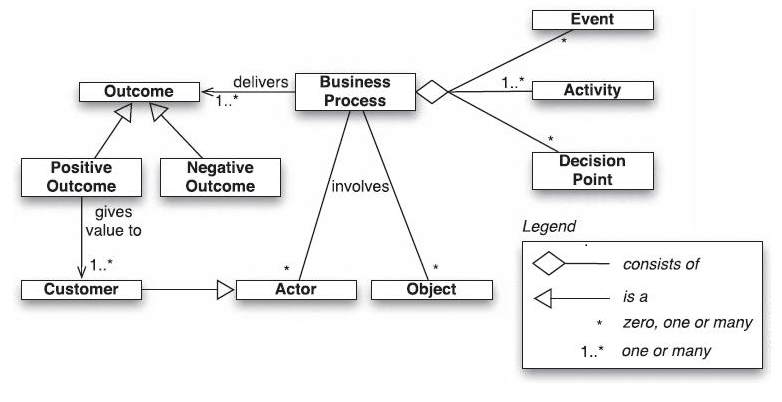
\includegraphics[scale=0.5]{Gambar/Bab-2/1-bp-components}
	\caption{Komponen BPM} 
	\label{komponenbp}
\end{figure}

\begin{description}
	\item{\textit{Event}} \hfill \\\textit{Event} adalah kejadian yang terjadi saat proses bisnis berjalan. 
	\item{\textit{Activity}} \hfill \\\textit{Activity} adalah kumpulan kegiatan yang dapat dikerjakan. Ketika suatu \textit{Activity} berupa sebuah kegiatan yang sederhana, \textit{activity} disebut dengan \textit{task}. 
	\item{\textit{Decision Point}} \hfill \\\textit{Decision point} adalah keputusan yang mempengaruhi proses selanjutnya.
	\item{\textit{Actor}} \hfill \\ \textit{Actor} berupa individu, organisasi, maupun sistem yang mempengaruhi proses bisnis. 
	\item{\textit{Object}} \hfill \\ \textit{Object} dapat berupa objek fisik (peralatan, bahan baku, produk, dokumen) maupun non fisik (dokumen elektronik, basis data elektronik).
	\item{\textit{Positive/Negative Outcome}} \hfill \\ Hasil dari bisnis proses dapat menghasilkan nilai bagi konsumen (positif) atau tidak menghasilkan nilai (negatif).
\end{description}




\subsection{Siklus \textit{Business Process Management}}
\label{sec:siklusBPM}
Suatu proses bisnis tidak selalu berjalan dengan baik. Banyak hal yang tidak diantisipasi sebelumnya dapat menggangu proses bisnis. Untuk menjaga kualitas dari sebuah proses bisnis diperlukan pengawasan dan kontrol pada suatu fase tertentu serta perbaikan apabila diperlukan. Maka dari itu, suatu bisnis proses dapat dilihat sebagai suatu siklus yang terus menerus meningkatkan kualitasnya. Siklus dalam proses bisnis berupa :
\begin{figure}[H]
	\centering
	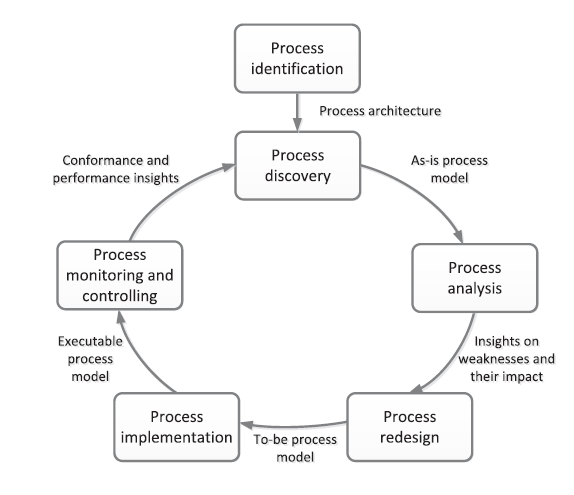
\includegraphics[scale=0.5]{Gambar/Bab-2/2-bpm-lifeCycle}
	\caption{Siklus BPM} 
	\label{siklusbpm}
\end{figure}

\begin{description}
	\item{\textit{Process Identification}} \hfill \\ Pada fase ini, suatu masalah bisnis ditemukan, kemudian proses-proses yang berhubungan dengan masalah bisnis tersebut diidentifikasi, dibatasi, dan dihubungkan satu sama lain. Proses ini terbagi menjadi dua tahap, yaitu \textit{designation} dan \textit{evaluation}. Tahap \textit{designation} bertujuan untuk mengenali proses-proses yang ada dan hubungan antar proses tersebut. Sedangkan tahap \textit{evaluation} memprioritaskan proses-proses yang menghasilkan nilai dan mempertimbangkan proses yang memiliki risiko atau tidak menghasilkan nilai. Fase ini menghasilkan arsitektur dari proses bisnis yang merepresentasikan proses bisnis dan relasi-relasinya.   
	\item{\textit{Process Discovery}} \hfill \\ Setiap proses yang relevan dengan masalah bisnis didokumentasikan, umumnya dalam bentuk model proses. Fase ini menghasilkan \textit{as-is process model}
	\item{\textit{Process Analysis}} \hfill \\ Pada fase ini, masalah pada model proses diidentifikasi, didokumentasikan, dan diukur kinerjanya dengan ukuran yang telah ditetapkan. Hasil dari fase ini adalah kumpulan masalah pada proses model.
	\item{\textit{Process Redesign}} \hfill \\ Tujuan dari fase ini adalah membuat perubahan pada proses yang dapat mengatasi berbagai kumpulan masalah yang telah diidentifikasi pada fase sebelumnya. Proses ini menghasilkan \textit{to-be process model}.
	\item{\textit{Process Implementation}} \hfill \\ Pada fase ini, model proses diimplementasikan untuk diekseskusi menggunakan \textit{Business Process Management System}.
	\item{\textit{Process Monitoring and Controlling}} \hfill \\ Setelah proses bisnis berjalan pada BPMS, berbagai data yang relevan dikumpulkan dan dianalisa untuk menentukan kualitas dari proses. Apabila terdapat masalah baru yang ditemukan, maka proses diulangi.
\end{description}



\section{\textit{Business Process Model Notation}}
\label{sec:bpmn}
Business Process Model Notation (BPMN) adalah notasi grafis yang menggambarkan langkah-langkah dalam proses bisnis. Notasi-notasi tersebut terdiri dari :

\subsection{\textit{Event}}
\label{sec:event}
Event merupakan kejadian yang terjadi pada proses bisnis yang dilambangkan dengan bentuk lingkaran. Notasi event secara umum terbagi menjadi tiga, yaitu \textit{start event, intermediate event,} dan \textit{end event}. \textit{Start event} menunjukkan dimulainya proses, \textit{intermediate event} dapat muncul ketika proses berjalan, sedangkan \textit{end event} menunjukkan berakhirnya proses.  
\begin{figure}[H]
	\centering
	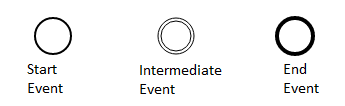
\includegraphics[scale=1]{Gambar/Bab-2/bpmn/event1}
	\caption{Notasi \textit{Event}} 
	\label{event}
\end{figure}

\subsection{\textit{Activity}}
\label{sec:activity}

\
\begin{figure}[H]
	\centering
	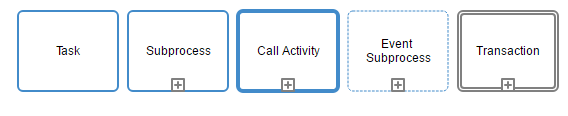
\includegraphics[scale=1]{Gambar/Bab-2/bpmn/activity}
	\caption{Notasi \textit{Activity}} 
	\label{activity}
\end{figure}

\subsection{\textit{Gateway}}
\label{sec:gateway}
\textit{Gateway} merupakan simbol yang menentukan percabangan dan penggabungan jalur dalam proses. Gateway dilambangakan dengan belah ketupat. Beberapa macam adalah :
\begin{itemize}
	\item \textit{Exclusive Gateway} (XOR) berarti memilih salah satu dari cabang yang ada. 
	\item \textit{Inclusive Gateway} berarti memilih satu, beberapa, atau seluruh cabang yang ada.
	\item \textit{Parallel Gateway} berarti mengerjakan proses pada seluruh cabang yang ada.
	\item \textit{Event Based} berarti mengerjakan proses setelah suatu \textit{event} selesai.
\end{itemize} 
\begin{figure}[H]
	\centering
	
\includegraphics[scale=1]{Gambar/Bab-2/bpmn/gateway}
	\caption{Notasi \textit{Gateway}} 
	\label{gateway}
\end{figure}


\subsection{\textit{Flow}}
\label{sec:flow}

\begin{figure}[H]
	\centering
	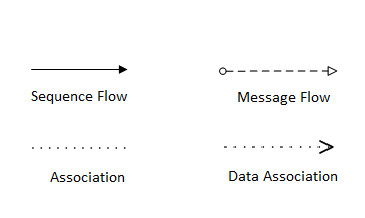
\includegraphics[scale=1]{Gambar/Bab-2/bpmn/flow}
	\caption{Notasi \textit{Flow}} 
	\label{flow}
\end{figure}

\subsection{\textit{Data}}
\label{sec:data}
\textit{Data Object} melambangkan informasi yang berjalan dalam proses seperti dokumen, e-mail, atau surat. Sedangkan \textit{Data Store} merupakan tempat proses membaca atau menyimpan data seperti basis data atau rak. 
\begin{figure}[H]
	\centering
	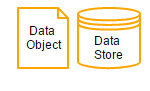
\includegraphics[scale=1]{Gambar/Bab-2/bpmn/data}
	\caption{Notasi \textit{Data}} 
	\label{data}
\end{figure}


\subsection{\textit{Artifact}}
\label{sec:artifacts}
\textit{Artifact} tidak mempengaruhi jalannya proses, tetapi hanya sebagai informasi tambahan agar proses lebih mudah dimengerti. Terdapat dua jenis, yaitu \textit{Text Annotation} dan \textit{Group}
\begin{figure}[H]
	\centering
	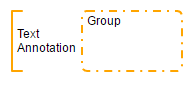
\includegraphics[scale=1]{Gambar/Bab-2/bpmn/artifact}
	\caption{Notasi \textit{Artifact} }
	\label{artifact}
\end{figure}


\subsection{\textit{Lanes} dan \textit{Pools}
\label{sec:poolslanes}

\begin{figure}[H]
	\centering
	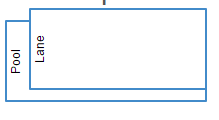
\includegraphics[scale=1]{Gambar/Bab-2/bpmn/swimlane}
	\caption{Notasi \textit{Lanes & Pools}} 
	\label{lanespools}
\end{figure}


 

\section{\textit{Business Process Management System (BPMS)}}
\textit{Business Process Management System (BPMS)} adalah sistem yang mengkoordinasikan otomatisasi proses bisnis. Tujuan dari BPMS adalah menyelesaikan proses pada waktu yang ditentukan dan menggunakan sumber daya yang tepat. 

\subsection{Arsitektur BPMS}
Komponen-komponen BPMS beserta hubungannya yang ditunjukkan pada Gambar ~\ref{fig:arsitekturbpms} terdiri dari :
\begin{itemize}
	\item \textit{Execution Engine}, menyediakan beberapa fungsi seperti mengeksekusi proses, mendistribusikan \textit{task}, mengambil dan menyimpan data yang diperlukan. 
	\item \textit{Process Modeling Tool}, \textit{tool} untuk membuat model proses.
	\item \textit{Worklist Handler}, me
	\item \textit{Administration & Monitoring Tool}
	\item \textit{Repository}
	\item \textit{Execution Logs}
\end{itemize}
\begin{figure}[H]
	\centering
	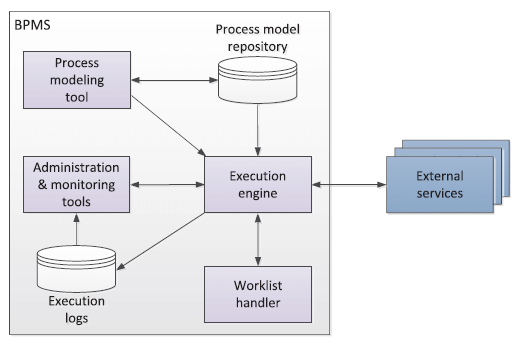
\includegraphics[scale=0.5]{Gambar/Bab-2/bpms/bpms}
	\caption{Arsitektur BPMS} 
	\label{fig:arsitekturbpms}
\end{figure}



\section{Camunda}
Camunda adalah \textit{framework} BPMS berbasis Java yang mendukung \textit{workflow} BPMN dan otomatisasi proses bisnis. 

\subsection{Arsitektur BPMS Camunda}
Camunda memiliki komponen-komponen yang sama dengan BPMS. 
\begin{figure}[H]
	\centering
	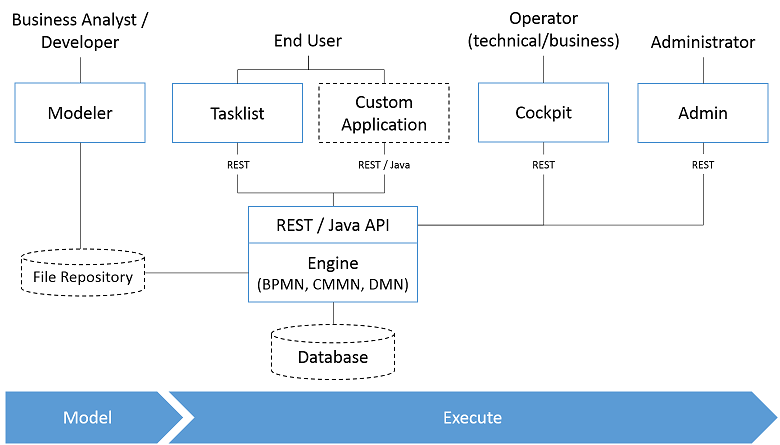
\includegraphics[scale=0.5]{Gambar/Bab-2/bpms/arsitektur-camunda}
	\caption{Arsitektur BPMS Camunda} 
	\label{fig:arsitekturcamunda}
\end{figure}


\section{Email}







		
	

 
\subsection{Kutipan}
\label{subs:kutipan} 
Berikut contoh kutipan dari berbagai sumber, untuk keterangan lebih lengkap, silahkan membaca file referensi.bib yang disediakan juga di template ini.
Contoh kutipan:
\begin{itemize}
	\item Buku:~\cite{berg:08:compgeom} 
	\item Bab dalam buku:~\cite{kreveld:04:GIS}
	\item Artikel dari Jurnal:~\cite{buchin:13:median}
	\item Artikel dari prosiding seminar/konferensi:~\cite{kreveld:11:median}
	\item Skripsi/Thesis/Disertasi:~\cite{lionov:02:animasi}~\cite{wiratma:10:following}~\cite{wiratma:22:later}
	\item Technical/Scientific Report:~\cite{kreveld:07:watertight}
	\item RFC (Request For Comments):~\cite{RFC1654}
	\item Technical Documentation/Technical Manual:~\cite{Z.500}~\cite{unicode:16:stdv9}~\cite{google:16:and7}
	\item Paten:~\cite{webb:12:comm}
	\item Tidak dipublikasikan:~\cite{wiratma:09:median}~\cite{lionov:11:cpoly}
	\item Laman web:~\cite{erickson:03:cgmodel}  
	\item Lain-lain:~\cite{agung:12:tango}
\end{itemize}    
  
\subsection{Gambar}

Pada hampir semua editor, penempatan gambar di dalam dokumen \LaTeX{} tidak dapat dilakukan melalui proses {\it drag and drop}.
Perhatikan contoh pada file bab2.tex untuk melihat bagaimana cara menempatkan gambar.
Beberapa hal yang harus diperhatikan pada saat menempatkan gambar:
\begin{itemize}
	\item Setiap gambar {\bf harus} diacu di dalam teks (gunakan {\it field} {\sc label})
	\item {\it Field} {\sc caption} digunakan untuk teks pengantar pada gambar. Terdapat dua bagian yaitu yang ada di antara tanda $[$ dan $]$ dan yang ada di antara tanda $\{$ dan $\}$. Yang pertama akan muncul di Daftar Gambar, sedangkan yang kedua akan muncul di teks pengantar gambar. Untuk skripsi ini, samakan isi keduanya.
	\item Jenis file yang dapat digunakan sebagai gambar cukup banyak, tetapi yang paling populer adalah tipe {\sc png} (lihat Gambar~\ref{fig:ularpng}), tipe {\sc jpg} (Gambar~\ref{fig:ularjpg}) dan tipe {\sc pdf} (Gambar~\ref{fig:ularpdf})
	\item Besarnya gambar dapat diatur dengan {\it field} {\sc scale}.
	\item Penempatan gambar diatur menggunakan {\it placement specifier} (di antara tanda  $[$ dan $]$ setelah deklarasi gambar.
	Yang umum digunakan adalah {\bf H} untuk menempatkan gambar {\bf sesuai} penempatannya di file .tex atau  {\bf h} yang berarti "kira-kira" di sini. \\
	Jika tidak menggunakan {\it placement specifier}, \LaTeX{} akan menempatkan gambar secara otomatis untuk menghindari bagian kosong pada dokumen anda.
	Walaupun cara ini sangat mudah, hindarkan terjadinya penempatan dua gambar secara berurutan. 	
	\begin{itemize}
		\item Gambar~\ref{fig:ularpng} ditempatkan di bagian atas halaman, walaupun penempatannya dilakukan setelah penulisan 3 paragraf setelah penjelasan ini.
		\item Gambar~\ref{fig:ularjpg} dengan skala 0.5 ditempatkan di antara dua buah paragraf. Perhatikan penulisannya di dalam file bab2.tex!
		\item Gambar~\ref{fig:ularpdf} ditempatkan menggunakan {\it specifier} {\bf h}.
	\end{itemize}
\end{itemize}
 
\kant[14-15]
\begin{figure} 
	\centering  
	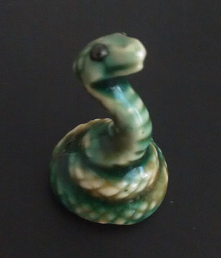
\includegraphics[scale=1]{ular-png}  
	\caption[Gambar {\it Serpentes} dalam format png]{Gambar {\it Serpentes} dalam format png} 
	\label{fig:ularpng} 
\end{figure} 

\kant[16]
\begin{figure}[H]
	\centering  
	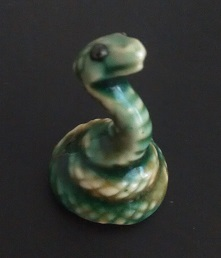
\includegraphics[scale=0.5]{ular-jpg}  
	\caption[Ular kecil]{Ular kecil} 
	\label{fig:ularjpg} 
\end{figure} 
\kant[17-19]

\begin{figure}[h] 
	\centering  
	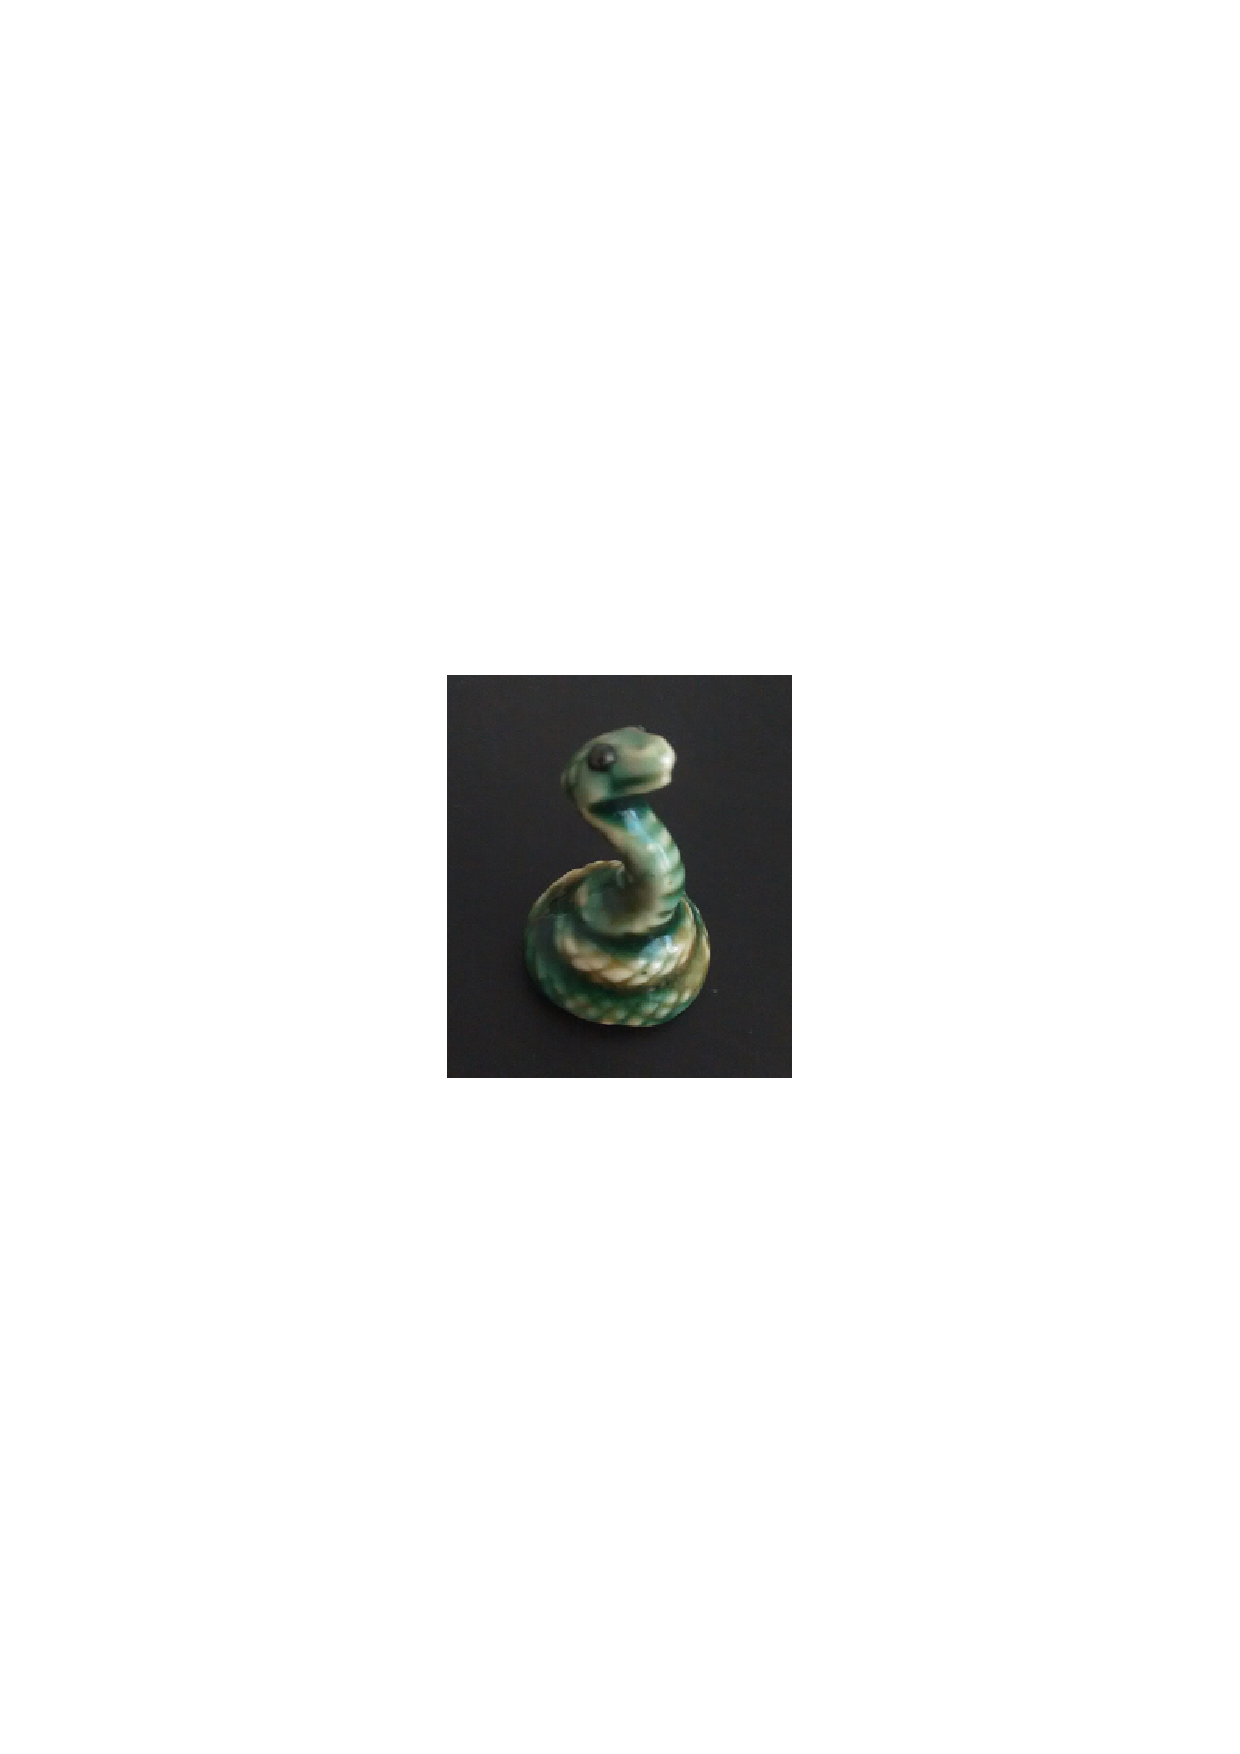
\includegraphics[scale=1]{ular-pdf}  
	\caption[ {\it Serpentes} betina]{ {\it Serpentes} jantan} 
	\label{fig:ularpdf} 
\end{figure} 
 
}{}
\ifdefstring{\vbabc}{1}{\chapter{Analisis}
\label{chap:analisis}
Bab ini berisi analisis BPMN dengan menggunakan skenario, analisis \textit{event} yang terkait dengan integrasi sistem email, dan mekanisme integrasi sistem email.
\section{Analisis BPMN}
\label{sec:analisisbpmn}

\subsection{Skenario Proposal Bisnis}
\label{skenario1}
John mempunyai ide proposal bisnis untuk manajernya, Peter. John menulis dan mengunggah proposal melalui sistem Camunda. Sebelum proposal disetujui, Peter harus memeriksa apakah proposalnya layak atau tidak. Jika proposalnya tidak layak, John harus memperbaiki dan mengunggahnya kembali. \textit{Workflow} dari skenario ini sebagai berikut :
		\begin{figure}[H]
			\centering
			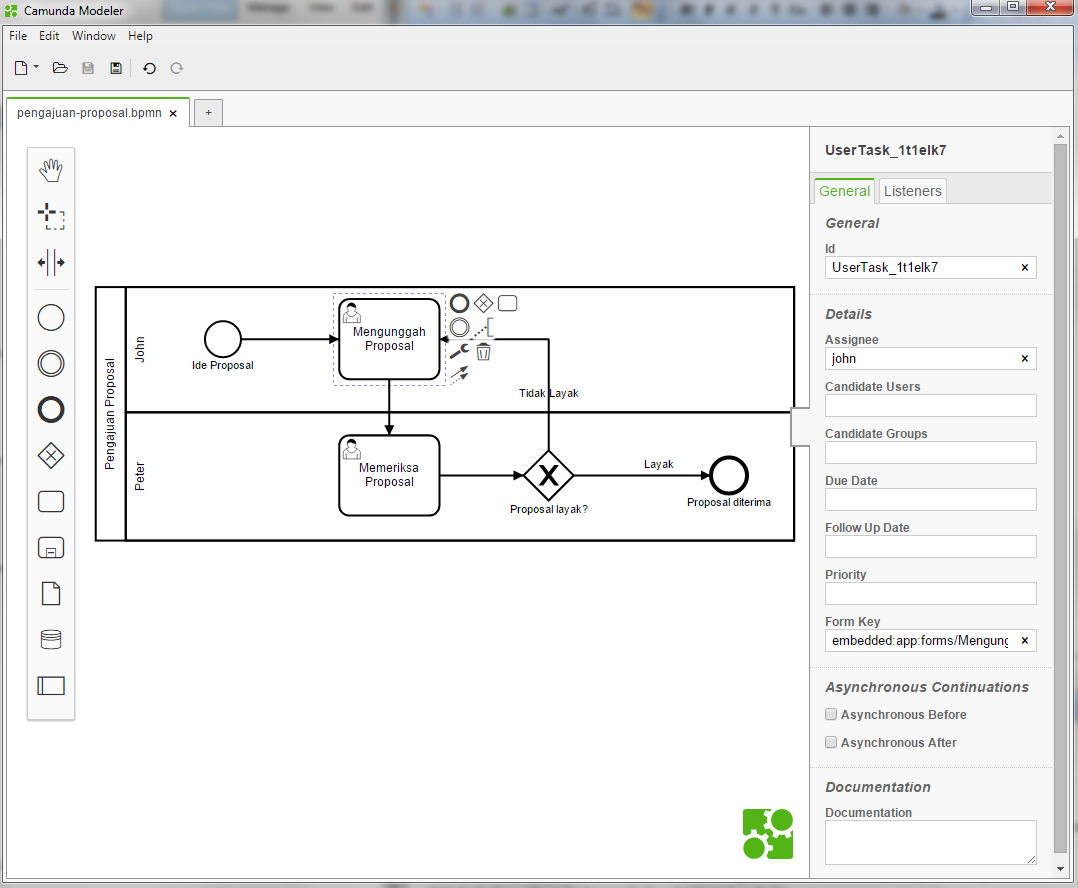
\includegraphics[scale=0.5]{Gambar/Bab-3/Kasus1-2}
			\caption{Mengunggah Proposal} 
			\label{fig:mengunggahproposal}
		\end{figure}
		
Pada Gambar ~\ref{fig:mengunggahproposal}, terdapat beberapa atribut yang memiliki nilai, yaitu :
\begin{itemize}
	\item Id, yaitu id dari \textit{task} yang dipilih
	\item Assignee, yaitu aktor yang akan mengerjakan \textit{task}
	\item Form Key, yaitu tautan ke file HTML yang berupa tampilan untuk mengunggah proposal.
\end{itemize}

\subsection{Skenario Proposal Bisnis dari Group}
\label{skenario2}
Pegawai di perusahaan X memiliki tiga divisi yaitu \textit{accounting}, \textit{sales}, dan \textit{management}. Divisi \textit{accounting} dan \textit{sales} dapat mengajukan proposal bisnis ke divisi \textit{management}. Sama seperti Skenario~\ref{skenario1}, divisi \textit{management} harus memeriksa apakah proposalnya layak atau tidak. Jika proposalnya tidak layak, pembuat proposal harus memperbaiki dan mengunggahnya kembali. Workflow dari skenario ini sebagai berikut :

		\begin{figure}[H]
			\centering
			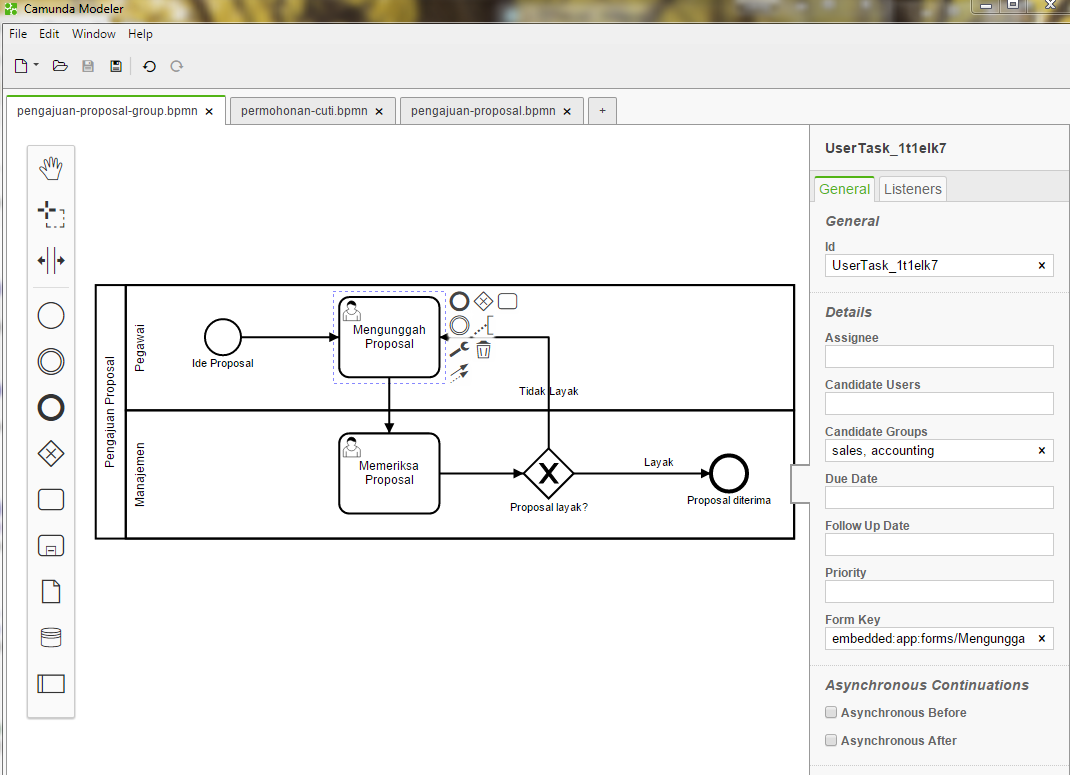
\includegraphics[scale=0.5]{Gambar/Bab-3/Kasus2-1}
			\caption{Mengunggah Proposal} 
			\label{fig:mengunggahproposalgroup}
		\end{figure}
Pada Gambar ~\ref{fig:mengunggahproposalgroup}, terdapat atribut \textit{Candidate Groups}. Atribut ini melambangkan bahwa \textit{task} ini dapat dikerjakan oleh salah satu anggota dari grup \textit{accounting} atau grup \textit{sales}.


\section{\textit{Event} yang Terkait dengan Integrasi Sistem Email}
\label{sec:eventUserTask}

Integrasi Camunda dengan sistem email pada skripsi ini bertujuan untuk memberi tahu aktor Camunda apabila ada \textit{tasks} yang perlu dikerjakan oleh aktor. Ketika aktor menerima email mengenai \textit{tasks} yang perlu dikejakan, aktor dapat langsung mengerjakannya. 

Camunda memiliki berbagai jenis \textit{tasks} seperti \textit{user tasks, manual tasks, service task}, dan lainnya. Karena proses integrasi email dengan Camunda melibatkan aktor (aktor menerima pemberitahuan pekerjaannya melalui email), \textit{task} yang akan diintegrasikan dengan sistem email adalah \textit{user tasks}.

\section{Mekanisme Integrasi Sistem Email}
\label{integrasi}
\textit{User tasks} memiliki atribut \textit{Task Listener} yang dapat mengeksekusi perintah. \textit{Task Listener} memiliki dua atribut, yaitu \textit{Event Type} dan \textit{Listener Type}. Terdapat empat pilihan dari \textit{Event Type}, yaitu \textit{create, assignment, complete, delete}. 
		\begin{figure}[H]
			\centering
			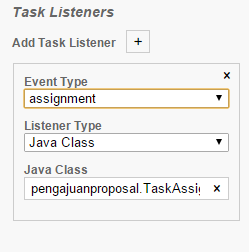
\includegraphics[scale=1]{Gambar/Bab-3/TaskListener}
			\caption{Event Task Listener} 
			\label{fig:eventtasklistener}
		\end{figure}
\begin{itemize}
	\item Create, perintah dieksekusi ketika \textit{task} telah dibuat dan siap untuk dikerjakan. 
	\item Assignment, perintah dieksekusi ketika aktor yang akan mengerjakan \textit{task} sudah ditentukan.
	\item Complete, perintah dieksekusi ketika \textit{task} sudah dikerjakan dan sebelum \textit{task} dihapus.
	\item Delete, perintah dieksekusi setelah \textit{task} dihapus.
\end{itemize}


Untuk mengintegrasikan \textit{user tasks} dengan email, \textit{event type} yang dapat digunakan adalah \textit{create} dan \textit{assignment}. \textit{Event complete} dan \textit{delete} tidak dapat digunakan untuk memberi tahu aktor karena setelah \textit{task} selesai dan dihapus, alamat email untuk \textit{Task} selanjutnya belum diambil sementara \textit{event} sudah selesai dipanggil.

Apabila menggunakan \textit{event create}, \textit{task} harus memiliki pemiliknya masing-masing ketika BPMN dibuat atau memiliki \textit{candidate user/group}. Bila pemilik \textit{task} belum ditentukan, email tidak akan terkirim, karena \textit{event create} sudah selesai dipanggil sebelum \textit{task} memiliki pemilik. Pengiriman email untuk \textit{task} yang belum memiliki aktor dapat menggunakan \textit{event create}. Sedangkan pada \textit{event assignment}, pengiriman email dilakukan setelah \textit{task} didelegasikan ke masing-masing user.




}{}
\ifdefstring{\vbabd}{1}{\chapter{Perancangan}
\label{chap:perancangan}
Untuk mempropagasi email, diperlukan perancangan sistem dan beberapa peran yang harus dilakukan oleh partisipan. 

\section{\textit{Event} yang Terkait dengan Integrasi Sistem Email}
\label{sec:eventUserTask}

Integrasi Camunda dengan sistem email pada skripsi ini bertujuan untuk memberi tahu aktor Camunda apabila ada \textit{tasks} yang perlu dikerjakan oleh aktor. Ketika aktor menerima email mengenai \textit{tasks} yang perlu dikejakan, aktor dapat langsung mengerjakannya. 

Camunda memiliki berbagai jenis \textit{tasks} seperti \textit{user tasks, manual tasks, service task}, dan lainnya. Karena proses integrasi email dengan Camunda melibatkan aktor (aktor menerima pemberitahuan pekerjaannya melalui email), \textit{task} yang akan diintegrasikan dengan sistem email adalah \textit{user tasks}.

\section{Mekanisme Integrasi Sistem Email}
\label{integrasi}
\textit{User tasks} memiliki atribut \textit{Task Listener} yang dapat mengeksekusi perintah. \textit{Task Listener} memiliki dua atribut, yaitu \textit{Event Type} dan \textit{Listener Type}. Terdapat empat pilihan dari \textit{Event Type}, yaitu \textit{create, assignment, complete, delete}. 
		\begin{figure}[H]
			\centering
			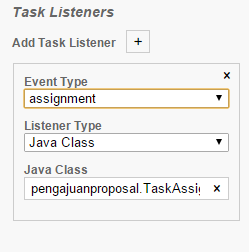
\includegraphics[scale=1]{Gambar/Bab-3/TaskListener}
			\caption{Event Task Listener} 
			\label{fig:eventtasklistener}
		\end{figure}
\begin{itemize}
	\item Create, perintah dieksekusi ketika \textit{task} telah dibuat dan siap untuk dikerjakan. 
	\item Assignment, perintah dieksekusi ketika aktor yang akan mengerjakan \textit{task} sudah ditentukan.
	\item Complete, perintah dieksekusi ketika \textit{task} sudah dikerjakan dan sebelum \textit{task} dihapus.
	\item Delete, perintah dieksekusi setelah \textit{task} dihapus.
\end{itemize}


Untuk mengintegrasikan \textit{user tasks} dengan email, \textit{event type} yang dapat digunakan adalah \textit{create} dan \textit{assignment}. \textit{Event complete} dan \textit{delete} tidak dapat digunakan untuk memberi tahu aktor karena setelah \textit{task} selesai dan dihapus, alamat email untuk \textit{Task} selanjutnya belum diambil sementara \textit{event} sudah selesai dipanggil.

Apabila menggunakan \textit{event create}, \textit{task} harus memiliki pemiliknya masing-masing ketika BPMN dibuat atau memiliki \textit{candidate user/group}. Bila pemilik \textit{task} belum ditentukan, email tidak akan terkirim, karena \textit{event create} sudah selesai dipanggil sebelum \textit{task} memiliki pemilik. Pengiriman email untuk \textit{task} yang belum memiliki aktor dapat menggunakan \textit{event create}. Sedangkan pada \textit{event assignment}, pengiriman email dilakukan setelah \textit{task} didelegasikan ke masing-masing user.





\section{Perancangan Sistem}
\label{rancangansistem}
Berdasarkan analisis di bab sebelumnya, maka untuk mempropagasi email diperlukan beberapa persyaratan, yaitu :
\begin{enumerate}
	\item Model proses menggunakan BPMN yang sudah dilengkapi form HTML untuk \textit{user task}, implementasi untuk \textit{service task} dan atribut lain yang diperlukan.
	\item Kumpulan \textit{user/group} yang akan mengerjakan tugas.
	\item Alamat email yang merepresentasikan sistem.
	\item Algoritma untuk mengirim email.
	\item Business Process Management System (BPMS), yaitu tools untuk mengotomasi jalannya proses.
\end{enumerate}

\subsection{Email}
\label{email}
Alamat email yang digunakan untuk merepresentasikan sistem berbasis Gmail SMTP. Gmail SMTP yang akan digunakan memiliki konfigurasi sebagai berikut \cite{smtpgoogle} :
\begin{itemize}
	\item Alamat server = smtp.gmail.com.
	\item Port = 587.
	\item Username Gmail.
	\item Password Gmail.
\end{itemize}
Email yang akan dikirimkan ke aktor memiliki format :
\begin{enumerate}
	\item Subjek :
	\item Nama aktor.
	\item Nama \textit{task}.
	\item Link ke \textit{task}, yaitu http://localhost/camunda/app/tasklist/default/\#/?task=(\textit{id task}).
\end{enumerate} 

\subsection{Algoritma Pengiriman Email}
\label{sec:algoritma}

Berikut adalah algoritma untuk mengirimkan email.
\begin{enumerate}
	\item Mengambil id dari \textit{task}.
	\item Mengambil email aktor yang akan mengerjakan \textit{task}.
	\item Membangkitkan subjek dan isi email yang berisi tautan ke task yang akan dikerjakan. Tautan didapatkan dari id \textit{task}.
	\item Membuat koneksi ke email server dengan \textit{username} dan \textit{password}
	\item Mengirim email.
\end{enumerate}


\section{Peran Partisipan}
\label{peranpartisipan}
Setiap partisipan memiliki perannya masing-masing. Desainer bertugas merancang BPMN, admin bertugas mengatur jalannya otomasi proses bisnis, sedangkan aktor bertugas mengerjakan \textit{tasks}
\subsection{Tugas Desainer}
\label{tugasdesainer}
Berdasarkan perancangan sistem di atas, seorang desainer model proses memiliki beberapa tugas, yaitu :
\begin{enumerate}
	\item Merancang model proses.
	\item Menambahkan form HTML pada \textit{user task}, \textit{implementasi service task}, \textit{task listener} untuk propagasi email, dan berbagai atribut lainnnya sesuai kebutuhan.
	\item Mendelegasikan task kepada user/group yang akan mengerjakan.
\end{enumerate}

\subsection{Tugas Admin}	
\label{tugasadmin}
\begin{enumerate}
	\item Membuat alamat email yang merepresentasikan sistem.
	\item Menambahkan \textit{username}, \textit{password}, dan \textit{host} email pada kode task listener yang berhubungan dengan propagasi email.
	\item Menambahkan user/group yang akan mengerjakan \textit{tasks} pada Camunda Admin.
	\item Menjalankan dan memulai proses.
\end{enumerate}

\subsection{Tugas Aktor}
\label{tugasaktor}
	\begin{enumerate}
	\item Memberitahu alamat email kepada admin.
	\item Mengerjakan \textit{task}.
\end{enumerate}


\subsection{Perancangan Aktor}
\label{perancanganaktor}
Untuk pengujian skenario, ada beberapa aktor yang dibuat, yaitu :
\begin{enumerate}
	\item John, dengan alamat email johncamunda@gmail.com dan bagian dari grup \textit{sales}.
	\item Mary, dengan alamat email marycamunda@gmail.com dan bagian dari grup \textit{accounting}.
	\item Peter, dengan alamat email petercamunda@gmail.com dan bagian dari grup \textit{management}.
\end{enumerate}}{}  
\ifdefstring{\vbabe}{1}{\chapter{Implementasi dan Pengujian}
\label{chap:implementasipengujian}
Pada bab ini akan diimplementasikan kode program untuk propagasi email dan pengujian dua skenario yang ada pada Bab ~\ref{chap:hasilstudi}.

\section{Lingkungan Implementasi}
\label{sec:lingkunganimplementasi}
Implementasi dilakukan pada lingkungan :
\begin{enumerate}
	\item Eclipse 4.5 Mars
	\item BPMN versi 2.0 dan Camunda Modeler versi 1.7.2.
	\item BPMS Camunda versi 7.6.0 dan berjalan pada tomcat versi 8.0.24.
	
\end{enumerate}

\section{Implementasi Algoritma Pengiriman Email}
\label{implementasialgo}
Beberapa potongan kode di bawah ini adalah kode untuk pengiriman email. Kode secara keseluruhan dapat dilihat pada Lampiran~\ref{lamp:tasklistener}
\begin{itemize}
	\item Konfigurasi email admin.
\begin{lstlisting}[language=Java,basicstyle=\tiny,caption=TaskAssignmentListener.java]
  private static final String HOST = "smtp.gmail.com";
  private static final String USER = "camundasys@gmail.com";
  private static final String PWD = "epW3S4KN";
\end{lstlisting}
	

	\item Kode untuk mengambil assignee (aktor dari \textit{task}, mengambil id \textit{task}, dan mengambil alamat email aktor. Method notify() dipanggil ketika \textit{event listener} pada\textit{task} dipanggil. Misalnya suatu \textit{task} yang menggunakan \textit{event listener create} akan memanggil method notify() ketika \textit{task} dibuat.
	\begin{lstlisting}[language=Java,basicstyle=\tiny,caption=TaskAssignmentListener.java]

 public void notify(DelegateTask delegateTask) {
    String assignee = delegateTask.getAssignee();
    String taskId = delegateTask.getId();
\end{lstlisting}

	\item Konfigurasi SMTP Gmail.
	\begin{lstlisting}[language=Java,basicstyle=\tiny,caption=TaskAssignmentListener.java]

               props = System.getProperties();
               props.put("mail.smtp.port", "587");
               props.put("mail.smtp.auth", "true");
               props.put("mail.smtp.starttls.enable", "true");

\end{lstlisting}
	\item Kode untuk mendapatkan aktor apabila atribut assignee pada BPMN memiliki nilai.
	\begin{lstlisting}[language=Java,basicstyle=\tiny,caption =TaskAssignmentListener.java]
	if (assignee != null) {
      IdentityService identityService = Context.getProcessEngineConfiguration().getIdentityService();
      User user = identityService.createUserQuery().userId(assignee).singleResult();
      if (user != null) {
    	  this.sendEmail(user);
      }
    }
	\end{lstlisting}
	
		\item Kode untuk mendapatkan aktor apabila atribut assignee pada BPMN tidak memiliki nilai. Kode ini mengambil aktor yang pada \textit{Candidate User} atau \textit{Candidate Group}.
	\begin{lstlisting}[language=Java,basicstyle=\tiny,caption =TaskAssignmentListener.java]
	    	TaskEntity task = (TaskEntity)delegateTask;
    	List<IdentityLinkEntity> identityLinks = task.getIdentityLinks();
    	
    	for(IdentityLinkEntity link : identityLinks) {
    		if(link.getType().equals(IdentityLinkType.CANDIDATE)) {
    		    if(link.isUser()) {
	    		     User user = Context.getProcessEngineConfiguration().getIdentityService().createUserQuery().userId(link.getUserId()).singleResult();
	    		     sendEmail(user);
    		    }
    		    if(link.isGroup()) {
    		        List<User> users = Context.getProcessEngineConfiguration().getIdentityService().createUserQuery().memberOfGroup(link.getGroupId()).list();
    		        for(User user : users) {
    		        	sendEmail(user);
    		        }
    		    }
    		}
    	}
	\end{lstlisting}
	
	

	\item Kode untuk membangkitkan subjek dan isi email. Kelas Properties menyimpan konfigurasi email yang akan digunakan. 
	\begin{lstlisting}[language=Java,basicstyle=\tiny,caption=TaskAssignmentListener.java]
 props = System.getProperties();
          props.put("mail.smtp.port", "587");
          props.put("mail.smtp.auth", "true");
          props.put("mail.smtp.starttls.enable", "true");
					
 session = Session.getDefaultInstance(props, null);
               message = new MimeMessage(session);
               message.addRecipient(Message.RecipientType.TO, new InternetAddress(recipient));
               message.setSubject("Task " + delegateTask.getName());
               
String name = user.getFirstName();
          String emailBody ="";
          emailBody += "Dear "+name+",<br>";
          emailBody += "Anda mendapatkan task " +taskName + " untuk dikerjakan.<br>";
          emailBody += "Segera akses http://localhost:1234/camunda/app/tasklist/default/#/?task="+taskId +" untuk menjalankannya.<br>";
          emailBody += "Terima kasih.";
          message.setContent(emailBody, "text/html");

\end{lstlisting}

	\item Kode untuk mengirimkan email.
	\begin{lstlisting}[language=Java,basicstyle=\tiny,caption=TaskAssignmentListener.java]

Transport transport = session.getTransport("smtp");            
               transport.connect(HOST, USER, PWD);
               transport.sendMessage(message, message.getAllRecipients());
               transport.close();
\end{lstlisting}
	
\end{itemize}
Implementasi algoritma pengiriman email (TaskAssignmentListener.java) dikaitkan dengan setiap \textit{user task} pada BPMN menggunakan \textit{event create}. Contohnya adalah sebagai berikut :
	\begin{figure}[H]
			\centering
			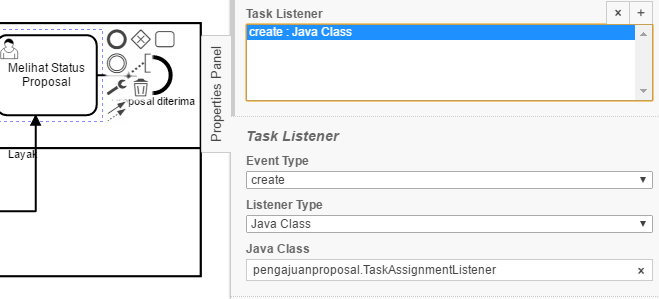
\includegraphics[scale=0.8]{Gambar/Bab-5/taskListener}
			\caption{Task Listener pada BPMN} 
			\label{fig:pengujian_taskListener}
	\end{figure}




\section{Pengujian}
\label{sec:pengujian}
Pengujian dilakukan pada skenario yang ada pada subbab \ref{hasilstudi_bpmn_masalah} Masalah Proses Bisnis. Ada dua skenario yang diuji, yaitu Pengajuan Proposal dan Pendaftaran BPJS. Kriteria yang diuji adalah berhasil atau tidaknya pengiriman email dan lama pengiriman email.

\subsection{Pengujian Kasus Pengajuan Proposal}
\label{pengujian_kasus1}
Workflow Pengajuan Proposal dapat dilihat pada subbab \ref{hasilstudi_workflow}
\begin{enumerate}
	\item Memulai proses Pengajuan Proposal pada 2:18 PM
		\begin{figure}[H]
			\centering
			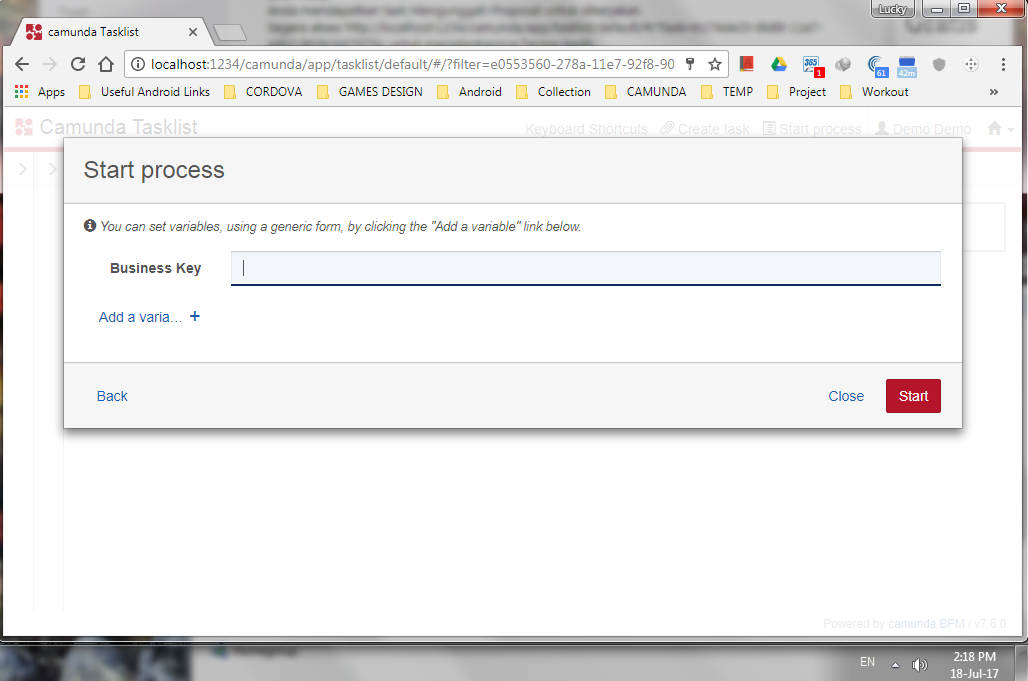
\includegraphics[scale=0.5]{Gambar/Bab-5/kasus1/1}
			\caption{Memulai Proses Pengajuan Proposal} 
			\label{fig:pengujian_kasus1_1}
	\end{figure}
	
		\item John dan Mary menerima email untuk mengunggah proposal pada 2:18 PM
		\begin{figure}[H]
			\centering
			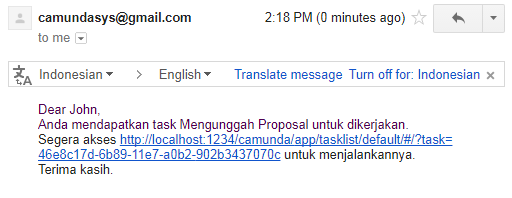
\includegraphics[scale=0.8]{Gambar/Bab-5/kasus1/2}
			\caption{Email Mengunggah Proposal} 
			\label{fig:pengujian_kasus1_2}
	\end{figure}
	
		\begin{figure}[H]
			\centering
			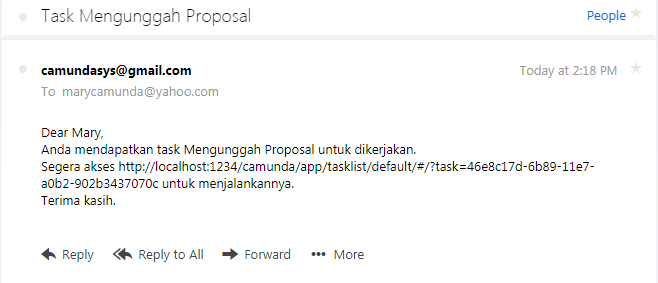
\includegraphics[scale=0.8]{Gambar/Bab-5/kasus1/3}
			\caption{Email Mengunggah Proposal} 
			\label{fig:pengujian_kasus1_3}
	\end{figure}
	
		\item John mengklaim \textit{task} dan mengunggah proposal pada 2:21 PM 
		\begin{figure}[H]
			\centering
			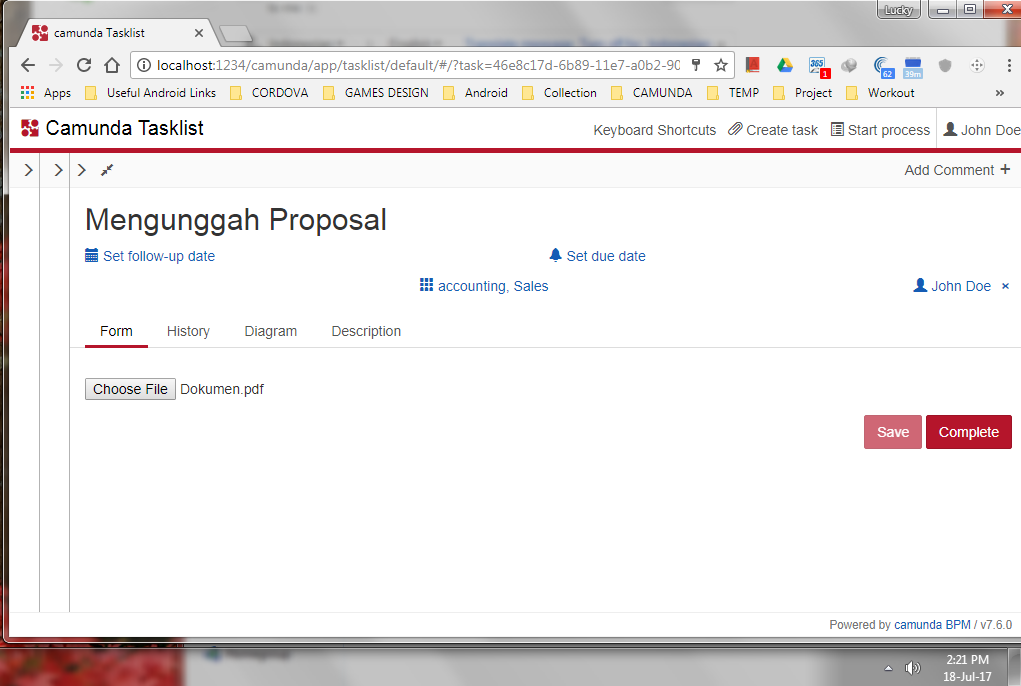
\includegraphics[scale=0.5]{Gambar/Bab-5/kasus1/4}
			\caption{Mengunggah Proposal} 
			\label{fig:pengujian_kasus1_4}
	\end{figure}
	
		\item Peter menerima email untuk memeriksa proposal pada 2:21 PM
		\begin{figure}[H]
			\centering
			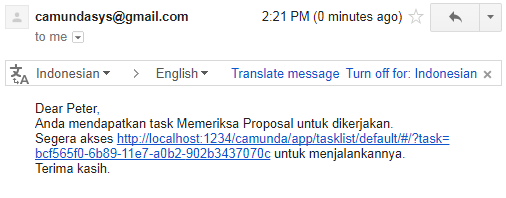
\includegraphics[scale=0.8]{Gambar/Bab-5/kasus1/5}
			\caption{Email Memeriksa Proposal} 
			\label{fig:pengujian_kasus1_5}
	\end{figure}
	
		\item Peter memeriksa proposal pada 2:23 PM
		\begin{figure}[H]
			\centering
			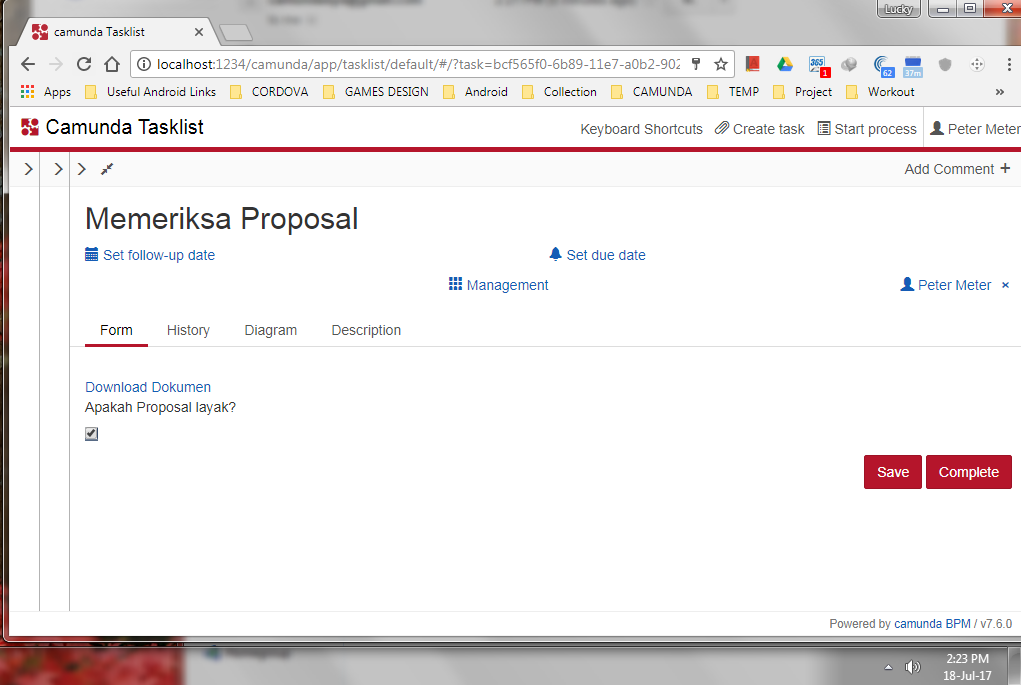
\includegraphics[scale=0.5]{Gambar/Bab-5/kasus1/6}
			\caption{Peter Memeriksa Proposal} 
			\label{fig:pengujian_kasus1_6}
	\end{figure}
	
		\item John menerima email untuk melihat status proposal pada 2:23 PM
		\begin{figure}[H]
			\centering
			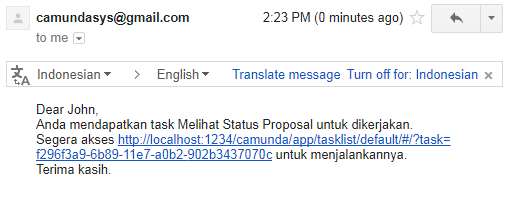
\includegraphics[scale=0.8]{Gambar/Bab-5/kasus1/7}
			\caption{Email Melihat Status Proposal} 
			\label{fig:pengujian_kasus1_7}
	\end{figure}
	
		\item John melihat status proposal pada 2:24 PM
		\begin{figure}[H]
			\centering
			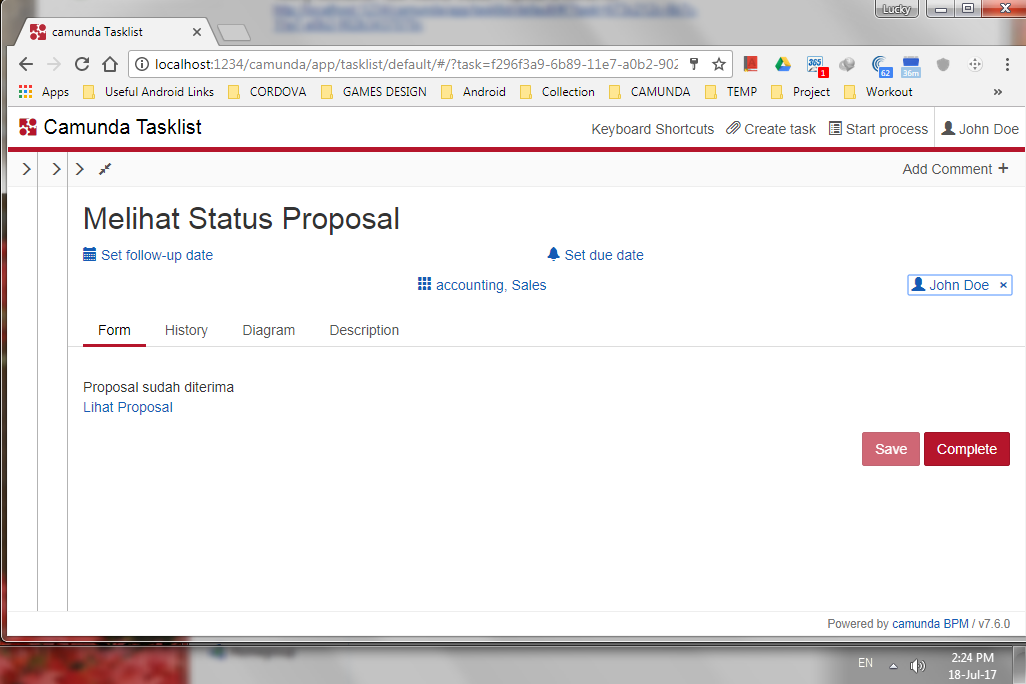
\includegraphics[scale=0.5]{Gambar/Bab-5/kasus1/8}
			\caption{John Melihat Status Proposal} 
			\label{fig:pengujian_kasus1_8}
	\end{figure}


\end{enumerate}



\subsection{Pengujian Kasus Pendaftaran BPJS}
\label{pengujian_kasus2}
Workflow Kasus Pendaftaran BPJS dapat dilihat pada subbab \ref{hasilstudi_workflow}
\begin{enumerate}
	\item Proses Pendaftaran BPJS dimulai pukul 2:40 PM.
			\begin{figure}[H]
			\centering
			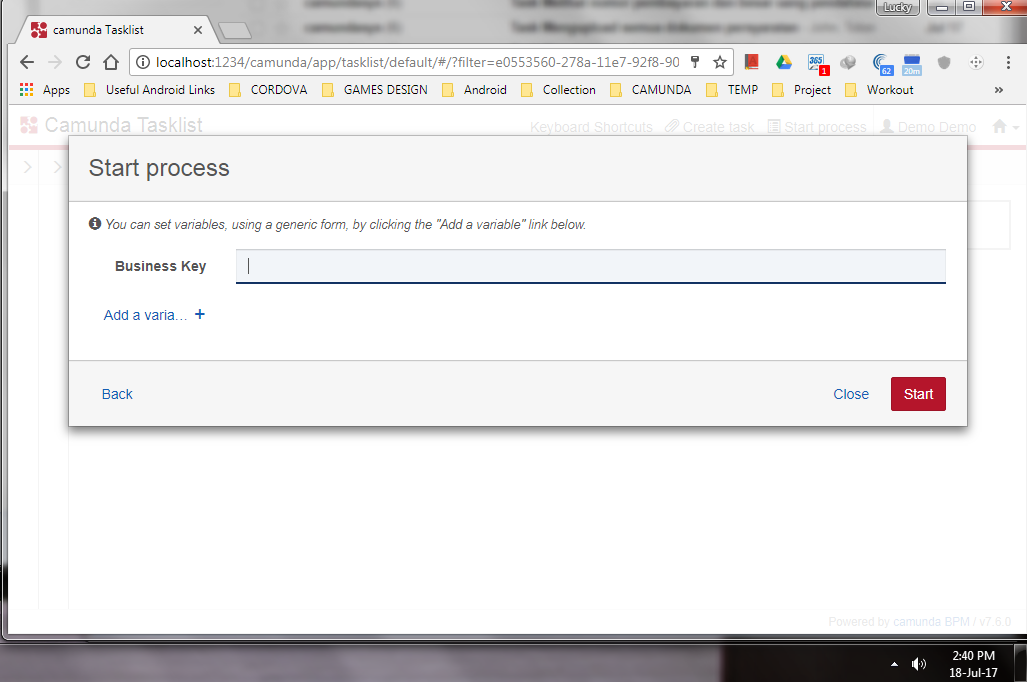
\includegraphics[scale=0.5]{Gambar/Bab-5/kasus2/1}
			\caption{Memulai Proses Pendaftaran BPJS} 
			\label{fig:pengujian_kasus2_1}
	\end{figure}
	

	\item John menerima email untuk mengisi formulir pendaftaran BPJS pada pukul 2:40PM.
			\begin{figure}[H]
			\centering
			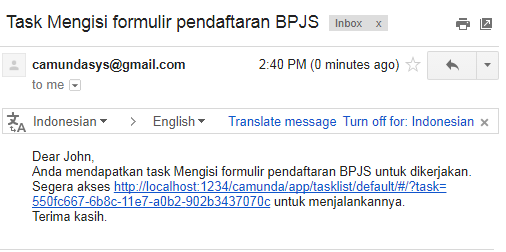
\includegraphics[scale=0.8]{Gambar/Bab-5/kasus2/2}
			\caption{Email Mengisi Formulir Pendaftaran BPJS} 
			\label{fig:pengujian_kasus2_2}
	\end{figure}
	

	\item John mengisi formulir pendaftaran BPJS pukul 2:41 PM
			\begin{figure}[H]
			\centering
			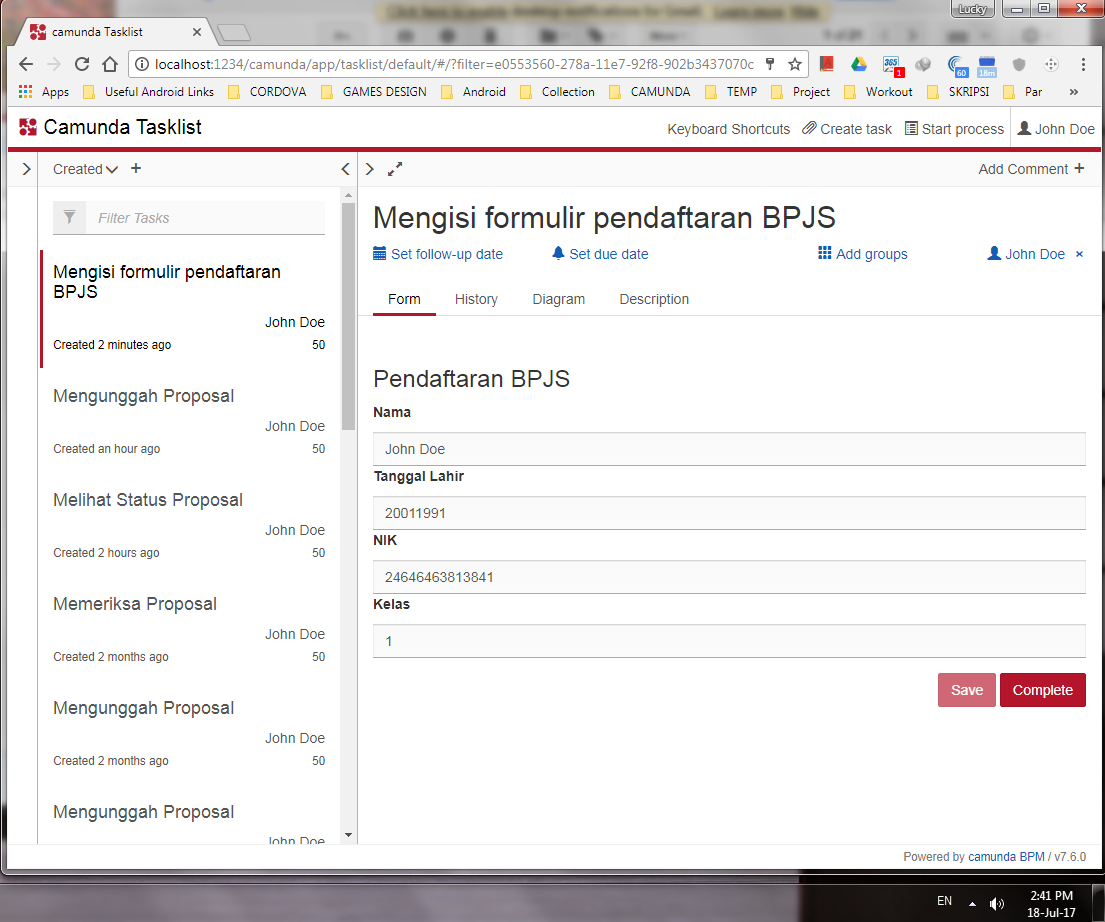
\includegraphics[scale=0.5]{Gambar/Bab-5/kasus2/3}
			\caption{Mengisi Formulir Pendaftaran BPJS} 
			\label{fig:pengujian_kasus2_3}
	\end{figure}
	

	\item John menerima email untuk mengunggah semua dokumen persyaratan pada pukul 2:42 PM.
			\begin{figure}[H]
			\centering 
			
\includegraphics[scale=0.8]{Gambar/Bab-5/kasus2/4}
			\caption{Email Mengunggah Dokumen Persyaratan} 
			\label{fig:pengujian_kasus2_4}
	\end{figure}
	

	\item John mengunggah semua dokumen persyaratan pada pukul 2:43 PM
			\begin{figure}[H]
			\centering
			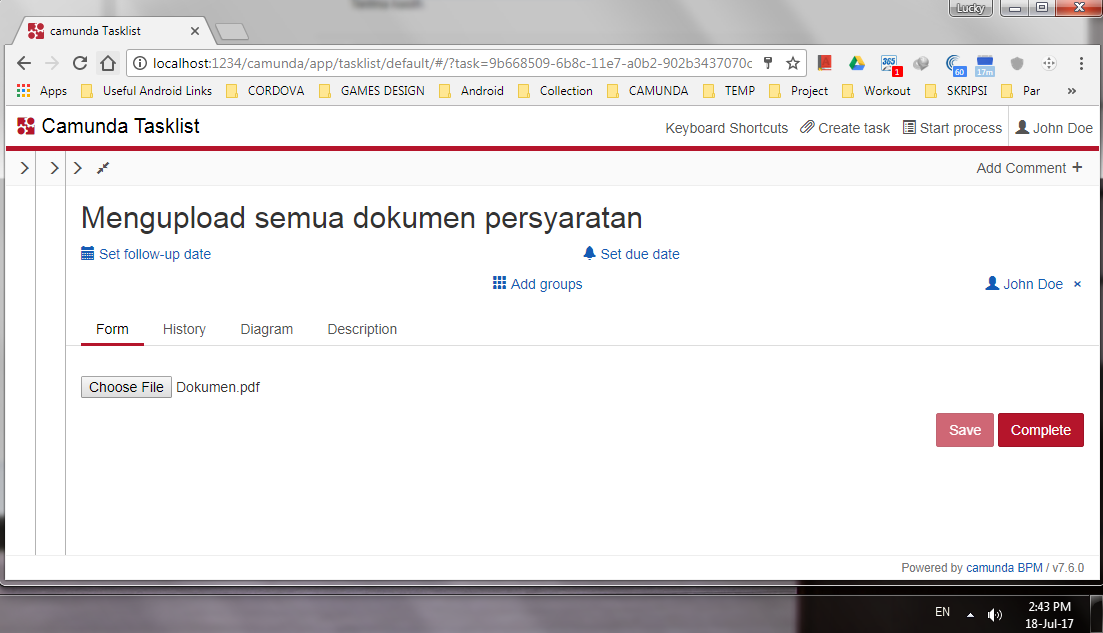
\includegraphics[scale=0.5]{Gambar/Bab-5/kasus2/5}
			\caption{Mengunggah Dokumen Persyaratan} 
			\label{fig:pengujian_kasus2_5}
	\end{figure}
	

	\item John menerima email untuk melihat nomor pembayaran dan besar uang pendaftaran pada pukul 2:43 PM
			\begin{figure}[H]
			\centering
			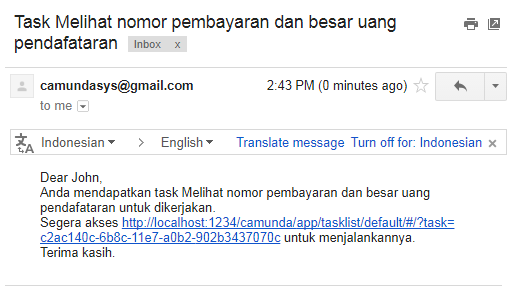
\includegraphics[scale=0.8]{Gambar/Bab-5/kasus2/6}
			\caption{Email Nomor Pembayaran dan Uang Pendaftaran} 
			\label{fig:pengujian_kasus2_6}
	\end{figure}
	

	\item John melihat nomor pembayaran dan besar uang pendaftaran pada pukul 2:44 PM
			\begin{figure}[H]
			\centering
			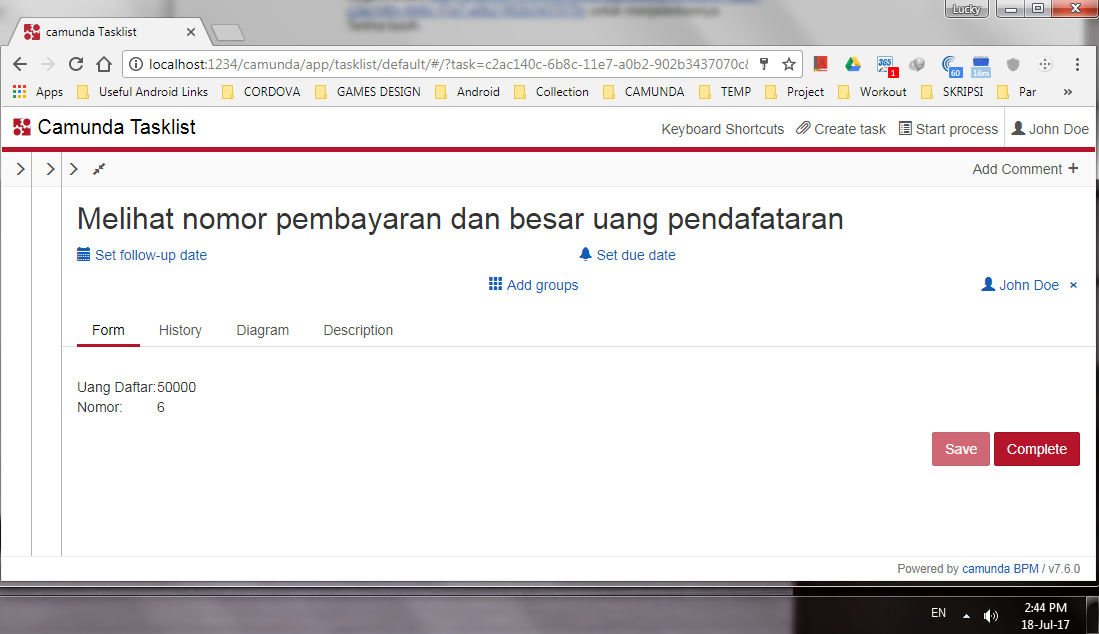
\includegraphics[scale=0.5]{Gambar/Bab-5/kasus2/7}
			\caption{Melihat Nomor Pembayaran dan Uang Pendaftaran} 
			\label{fig:pengujian_kasus2_7}
	\end{figure}
	

	\item John menerima email untuk memilih jadwal verifikasi dokumen pada pukul 2:43 PM
			\begin{figure}[H]
			\centering
			
\includegraphics[scale=0.8]{Gambar/Bab-5/kasus2/8}
			\caption{Email Memilih Jadwal Verifikasi Dokumen} 
			\label{fig:pengujian_kasus2_8}
	\end{figure}
	

	\item John memilih jadwal verifikasi dokumen pada pukul 2:44 PM
			\begin{figure}[H]
			\centering
			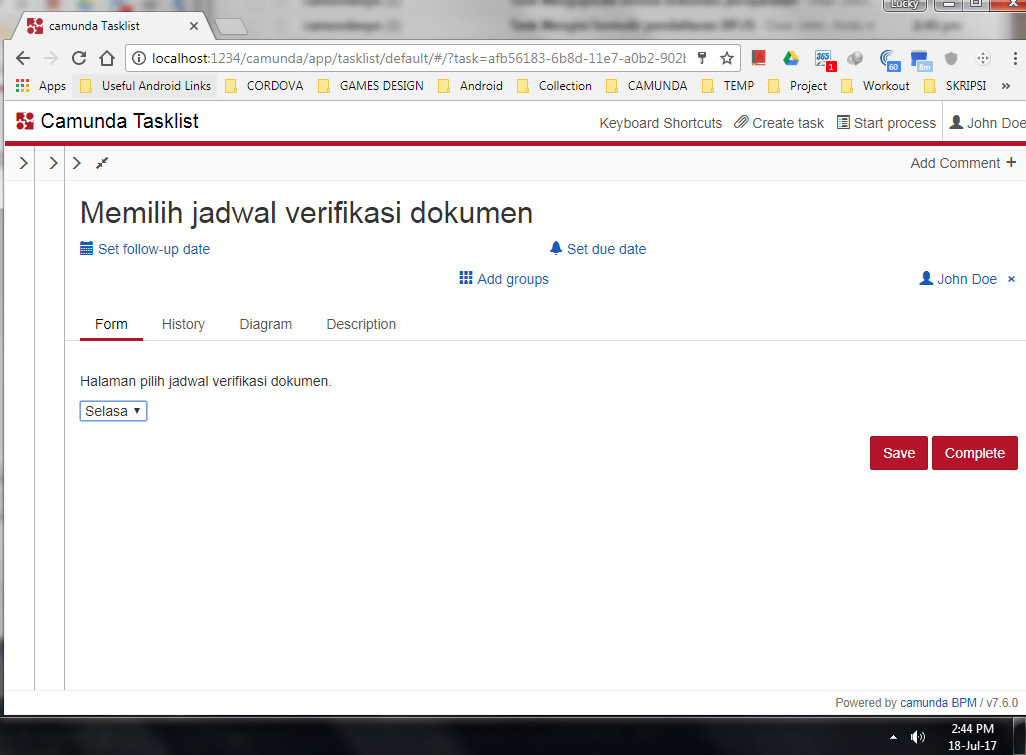
\includegraphics[scale=0.5]{Gambar/Bab-5/kasus2/9}
			\caption{Memilih Jadwal Verifikasi Dokumen} 
			\label{fig:pengujian_kasus2_9}
	\end{figure}
	

	\item John menerima email untuk mencetak jadwal dan nomor antrian pada pukul 2:44 PM
			\begin{figure}[H]
			\centering
			
\includegraphics[scale=0.8]{Gambar/Bab-5/kasus2/10}
			\caption{Email Mencetak Jadwal} 
			\label{fig:pengujian_kasus2_10}
	\end{figure}
	

	\item John mencetak jadwal dan nomor antrian pada pukul 2:46 PM
			\begin{figure}[H]
			\centering
			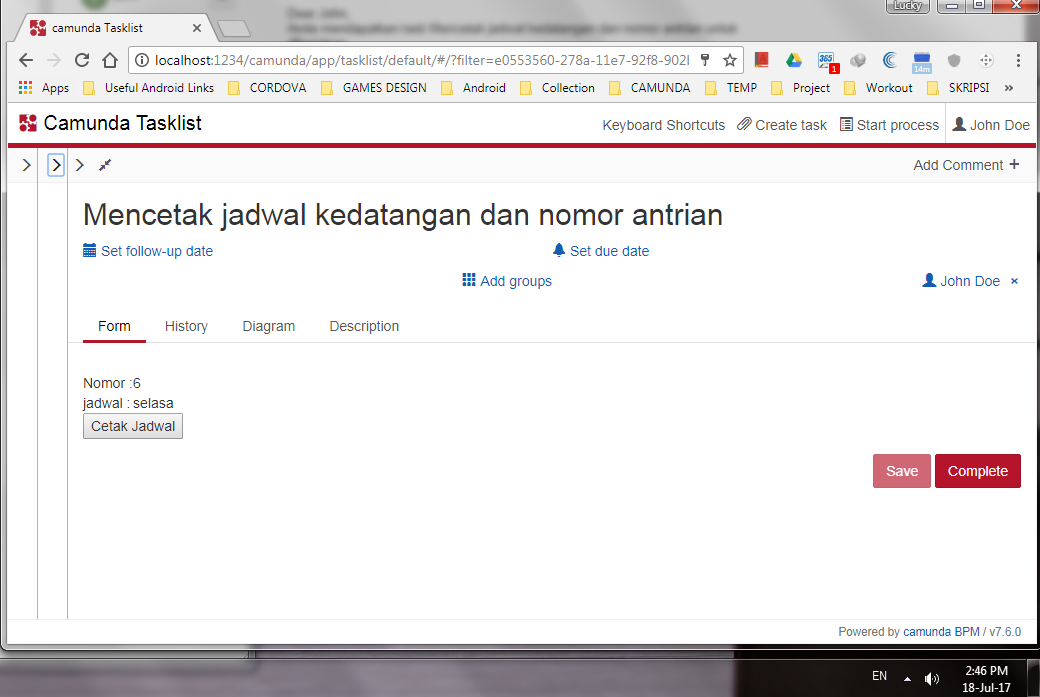
\includegraphics[scale=0.5]{Gambar/Bab-5/kasus2/11}
			\caption{Mencetak Jadwal dan Nomor Antrian} 
			\label{fig:pengujian_kasus2_11}
	\end{figure}
	

	\item Mary, sebagai petugas BPJS menerima email untuk memverifikasi pendaftaran pada pukul 2:46 PM
			\begin{figure}[H]
			\centering
			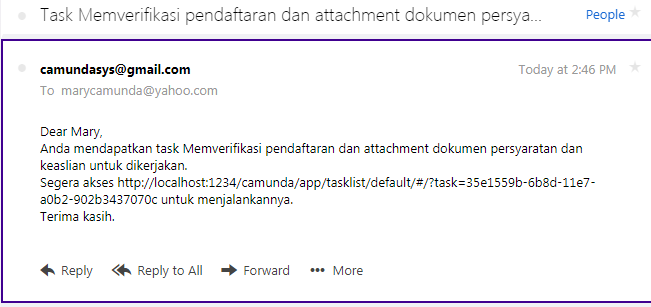
\includegraphics[scale=0.8]{Gambar/Bab-5/kasus2/12}
			\caption{Email Verifikasi Pendaftaran} 
			\label{fig:pengujian_kasus2_12}
	\end{figure}
	

	\item Mary memverifikasi pendaftaran dan semua persyaratan pada pukul 2:47 PM
			\begin{figure}[H]
			\centering
			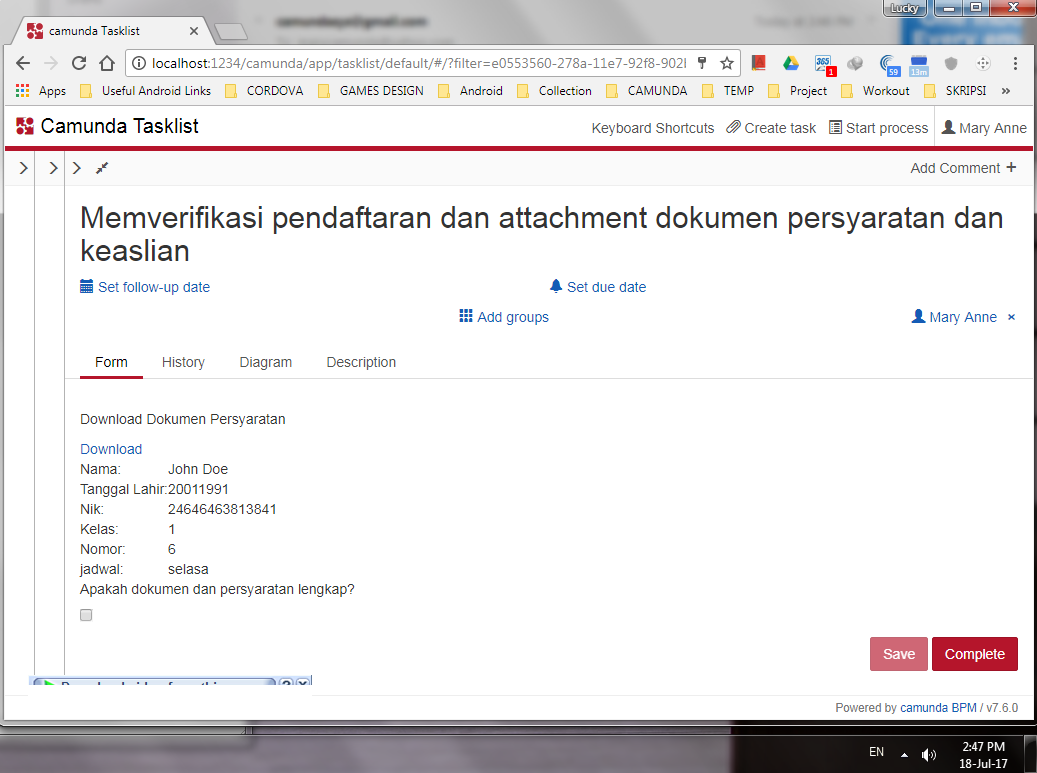
\includegraphics[scale=0.5]{Gambar/Bab-5/kasus2/13}
			\caption{Memverifikasi Pendaftaran dan Semua Persyaratan} 
			\label{fig:pengujian_kasus2_13}
	\end{figure}
	

	\item Mary menerima email untuk mencetak kartu BPJS pada pukul 2:47 PM
			\begin{figure}[H]
			\centering
			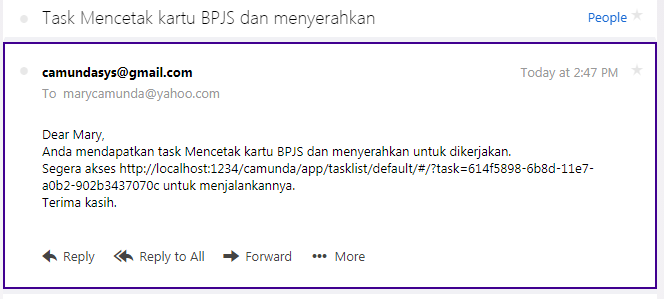
\includegraphics[scale=0.8]{Gambar/Bab-5/kasus2/14}
			\caption{Email Mencetak Kartu BPJS} 
			\label{fig:pengujian_kasus2_14}
	\end{figure}
	

	\item Mary mencetak kartu BPJS pada pukul 2:48 PM
			\begin{figure}[H]
			\centering
			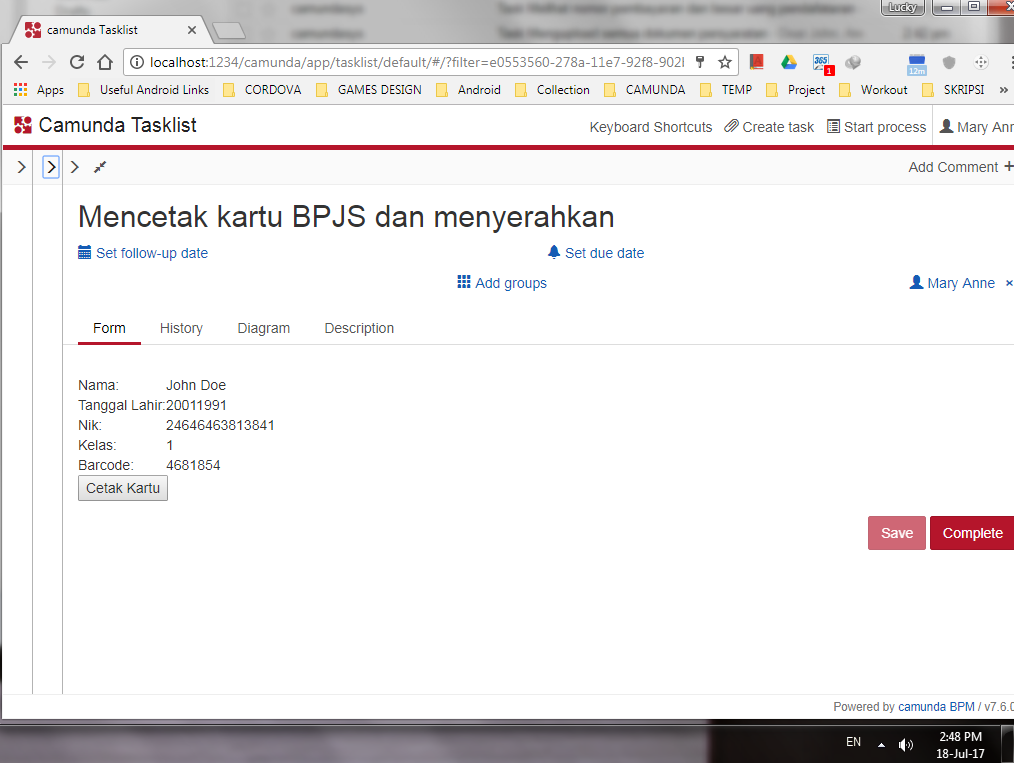
\includegraphics[scale=0.5]{Gambar/Bab-5/kasus2/15}
			\caption{Mencetak Kartu BPJS} 
			\label{fig:pengujian_kasus2_15}
	\end{figure}
\end{enumerate}





		

\section{Hasil Pengujian}
\label{hasilpengujian}
Berdasarkan pengujian dua kasus yang telah dilakukan (Pengajuan Proposal dan Pendaftaran BPJS), hasilnya adalah :
\begin{enumerate}
	\item Seluruh \textit{user task} mengirimkan email ke pemilik \textit{task}.
	\item Email langsung dikirim ke pemilik \textit{task} setelah \textit{task} siap dikerjakan. Dapat dilihat dari waktu \textit{task} sebelumnya selesai dan waktu email diterima oleh pemilik \textit{task} yang akan dikerjakan.
\end{enumerate}}{}
\ifdefstring{\vbabf}{1}{\chapter{Kesimpulan dan Saran}
\label{chap:kesimpulan_saran}
Pada bab enam ini akan dijelaskan mengenai kesimpulan dan saran yang didapat dari propagasi sistem email dengan Camunda 
\section{Kesimpulan}
\label{sec:kesimpulan}
Berdasarkan hasil pengembangan propagasi sistem email dengan Camunda, didapatkan beberapa kesimpulan sebagai berikut :
\begin{enumerate}
	\item \textit{Workflow} dapat dimodelkan sebagai BPMN yang dapat divisualisasikan oleh BPMS. 
	\item \textit{Event-event} dapat dipropagasi via email sehingga aktor dapat mengetahui apabila ada \textit{task} yang harus dikerjakan. Dengan demikian akan meningkatkan efektifitas dan efisiensi proses bisnis.
	\item \textit Propagasi email dapat dilakukan dengan cara menyisipkan \textit{Task Listener} di event yang akan dipropagasi. Selain itu dibutuhkan peran admin untuk mendaftarkan alamat email aktor.
	\item \textit Pengujian telah dilakukan dengan dua skenario yaitu Pengajuan Proposal dan Pendaftaran BPJS. Berdasarkan subbab \ref{analisispengujian} Analisis Pengujian, didapati bahwa setiap \textit{user task} yang disisipkan \textit{TaskAssignmentListener.java} dapat mengirim email ke pemilik \textit{user task} masing-masing segera setelah \textit{task} siap untuk dikerjakan.
	

\end{enumerate}

\section{Saran}
\label{sec:saran}
Berdasarkan kesimpulan yang didapat, ada beberapa saran untuk penelitian dan pengembangan lebih lanjut, antara lain :
\begin{enumerate}
	\item Menambahkan statistik efektifitas proses bisnis.
	\item Aspek integrasi bisa ditambahkan dengan \textit{external tasks}, yaitu sistem di luar Camunda dengan memanfaatkan \textit{web service}.
\end{enumerate}}{}
\ifdefstring{\vbabg}{1}{\include{Bab/bab7}}{}
\ifdefstring{\vbabh}{1}{\include{Bab/bab8}}{}
\ifdefstring{\vbabi}{1}{\include{Bab/bab9}}{}

\bibliographystyle{compj} 
\bibliography{referensi}

\appendix
\apptoc 
 
\tampillmp{\vlmp}
\ifdefstring{\vlmpa}{1}{\chapter{Kode Program Pengiriman Email}
\label{lamp:tasklistener}

\begin{lstlisting}[language=Java,basicstyle=\tiny,caption=TaskAssignmentListener.java]

package pengajuanproposal;


import java.util.List;
import java.util.Properties;
import java.util.Set;
import java.util.logging.Level;
import java.util.logging.Logger;

import javax.mail.Address;
import javax.mail.Message;
import javax.mail.MessagingException;
import javax.mail.NoSuchProviderException;
import javax.mail.Session;
import javax.mail.Transport;
import javax.mail.internet.MimeMessage;
import javax.mail.internet.InternetAddress;

import org.camunda.bpm.engine.IdentityService;
import org.camunda.bpm.engine.delegate.DelegateTask;
import org.camunda.bpm.engine.delegate.TaskListener;
import org.camunda.bpm.engine.identity.User;
import org.camunda.bpm.engine.impl.context.Context;
import org.camunda.bpm.engine.impl.persistence.entity.IdentityLinkEntity;
import org.camunda.bpm.engine.impl.persistence.entity.TaskEntity;
import org.camunda.bpm.engine.task.IdentityLinkType;


public class TaskAssignmentListener implements TaskListener {
  private static final String HOST = "smtp.gmail.com";
  private static final String USER = "camundasys@gmail.com";
  private static final String PWD = "epW3S4KN";
  
  String assignee;
  String taskId;
  String taskName;
  
  String[] recipient;
  
  static Properties props;
  static Session session;
  static MimeMessage message;
  

  public void notify(DelegateTask delegateTask) {
    assignee = delegateTask.getAssignee();
    taskId = delegateTask.getId();
    taskName = delegateTask.getName();
    delegateTask.getCandidates();
    
    if (assignee != null) {
      IdentityService identityService = Context.getProcessEngineConfiguration().getIdentityService();
      User user = identityService.createUserQuery().userId(assignee).singleResult();
      if (user != null) {
    	  this.sendEmail(user);
      }
    }
    else{
    	TaskEntity task = (TaskEntity)delegateTask;
    	List<IdentityLinkEntity> identityLinks = task.getIdentityLinks();
    	
    	for(IdentityLinkEntity link : identityLinks) {
    		if(link.getType().equals(IdentityLinkType.CANDIDATE)) {
    		    if(link.isUser()) {
	    		     User user = Context.getProcessEngineConfiguration().getIdentityService().createUserQuery().userId(link.getUserId()).singleResult();
	    		     sendEmail(user);
    		    }
    		    if(link.isGroup()) {
    		        List<User> users = Context.getProcessEngineConfiguration().getIdentityService().createUserQuery().memberOfGroup(link.getGroupId()).list();
    		        for(User user : users) {
    		        	sendEmail(user);
    		        }
    		    }
    		}
    	}
    }
  }
  
  public void sendEmail(User user){
      try {
          props = System.getProperties();
          props.put("mail.smtp.port", "587");
          props.put("mail.smtp.auth", "true");
          props.put("mail.smtp.starttls.enable", "true");

          
          session = Session.getDefaultInstance(props, null);
          message = new MimeMessage(session);
          message.addRecipient(Message.RecipientType.TO, new InternetAddress(user.getEmail()));
          message.setSubject("Task " + taskName);
          
          String emailBody = user.getFirstName() +",<br>";
          emailBody += "Tolong Selesaikan Task " +taskName + " di bawah ini.<br>";
          emailBody += "http://localhost:1234/camunda/app/tasklist/default/#/?task="+taskId;
          message.setContent(emailBody, "text/html");
          

          Transport transport = session.getTransport("smtp");            
          transport.connect(HOST, USER, PWD);
          transport.sendMessage(message, message.getAllRecipients());
          transport.close();
      } catch (NoSuchProviderException ex) {
          Logger.getLogger(TaskAssignmentListener.class.getName()).log(Level.SEVERE, null, ex);
      } catch (MessagingException ex) {
          Logger.getLogger(TaskAssignmentListener.class.getName()).log(Level.SEVERE, null, ex);
      }
  }

}


\end{lstlisting}
}{}
\ifdefstring{\vlmpb}{1}{\chapter{Kode pom.xml}
\label{lamp:pom}

\begin{lstlisting}[language=xml,basicstyle=\tiny,caption=pom.xml]
<project xmlns="http://maven.apache.org/POM/4.0.0" xmlns:xsi="http://www.w3.org/2001/XMLSchema-instance"
         xsi:schemaLocation="http://maven.apache.org/POM/4.0.0 http://maven.apache.org/xsd/maven-4.0.0.xsd">
  <modelVersion>4.0.0</modelVersion>
  <groupId>org.camunda.bpm.getstarted</groupId>
  <artifactId>loan-approval</artifactId>
  <version>0.1.0-SNAPSHOT</version>
  <packaging>war</packaging>

  <dependencyManagement>
    <dependencies>
      <dependency>
        <groupId>org.camunda.bpm</groupId>
        <artifactId>camunda-bom</artifactId>
        <version>7.6.0</version>
        <scope>import</scope>
        <type>pom</type>
      </dependency>
    </dependencies>
  </dependencyManagement>

  <dependencies>
    <dependency>
      <groupId>org.camunda.bpm</groupId>
      <artifactId>camunda-engine</artifactId>
      <scope>provided</scope>
    </dependency>

    <dependency>
      <groupId>javax.servlet</groupId>
      <artifactId>javax.servlet-api</artifactId>
      <version>3.0.1</version>
      <scope>provided</scope>
    </dependency>
  </dependencies>

  <build>
    <plugins>
      <plugin>
        <groupId>org.apache.maven.plugins</groupId>
        <artifactId>maven-war-plugin</artifactId>
        <version>2.3</version>
        <configuration>
          <failOnMissingWebXml>false</failOnMissingWebXml>
        </configuration>
      </plugin>
    </plugins>
  </build>

</project>

\end{lstlisting}}{}
\ifdefstring{\vlmpc}{1}{\chapter{Kode Skenario}
\label{lamp:kodeskenario}

\section{Kasus 1 - Pengajuan Proposal}
\label{sec:kodekasus1}
\begin{lstlisting}[language=Java,basicstyle=\tiny,caption=PengajuanProposal.java]
package pengajuanproposal;

import org.camunda.bpm.application.ProcessApplication;
import org.camunda.bpm.application.impl.ServletProcessApplication;

@ProcessApplication("PengajuanProposal App")
public class PengajuanProposal extends ServletProcessApplication{

}
\end{lstlisting}

\begin{lstlisting}[language=html,basicstyle=\tiny,caption=MengunggahProposal.html]
<html>
<head>
<body>
	<form method="post" name="upload-dokumen">
		<input type="file"
       cam-variable-name="proposal"
       cam-variable-type="File"
       cam-max-filesize="10000000"/>
	</form>
</body>
</html>
\end{lstlisting}

\begin{lstlisting}[language=html,basicstyle=\tiny,caption=MemeriksaProposal.html]
<html>
<head></head>

<body>
<form role="form" name="form">
  	<a cam-file-download="proposal">Download Dokumen</a>
    <p>Apakah Proposal layak?</p>
    <input cam-variable-name="valid"
             cam-variable-type="Boolean"
             type="checkbox"
             name="valid"
             class="form-control" />
    
</form> 
</body>
</html>
\end{lstlisting}


\begin{lstlisting}[language=html,basicstyle=\tiny,caption=MelihatStatusProposal.html]
<html>
	<head></head>
	<body>
	<h> Proposal sudah diterima </h>
	
	<form role="form" name="form">
  	<a cam-file-download="proposal">Lihat Proposal</a>
  	</form>
	


</html>
\end{lstlisting}

\section{Kasus 2 - Pendaftaran BPJS}
\label{sec:kode_kasus2}
\begin{lstlisting}[language=Java,basicstyle=\tiny,caption=PendaftaranBPJS.java]
package pengajuanproposal;

package org.camunda.bpm.getstarted.pendaftaranbpjs;

import org.camunda.bpm.application.ProcessApplication;
import org.camunda.bpm.application.impl.ServletProcessApplication;

@ProcessApplication("PendaftaranBPJS App")
public class PendaftaranBPJS extends ServletProcessApplication {
	
}

\end{lstlisting}

\begin{lstlisting}[language=Java,basicstyle=\tiny,caption=PembangkitBarcode.java]
package org.camunda.bpm.getstarted.pendaftaranbpjs;

import java.util.Random;

import org.camunda.bpm.engine.delegate.DelegateExecution;
import org.camunda.bpm.engine.delegate.JavaDelegate;

public class PembangkitBarcode implements JavaDelegate{

	public int getBarcode(){
		Random rand = new Random();
		int nomor = rand.nextInt(10000000)+100000;
		return nomor;
	}
	
	public void execute(DelegateExecution execution) throws Exception {
		String barcode = ""+this.getBarcode();
		execution.setVariable("barcode", barcode);
	}
}

\end{lstlisting}

\begin{lstlisting}[language=Java,basicstyle=\tiny,caption=PembangkitJadwal.java]
package org.camunda.bpm.getstarted.pendaftaranbpjs;

import java.util.Random;
import java.util.logging.Logger;

import org.camunda.bpm.engine.delegate.DelegateExecution;
import org.camunda.bpm.engine.delegate.JavaDelegate;
import org.camunda.bpm.engine.runtime.ProcessInstance;

public class PembangkitJadwal implements JavaDelegate{
	public final static Logger LOGGER = Logger.getLogger("pembangkit-jadwal");
	public String jadwalKedatangan(Object hari){
		
		return hari+"";
	}
	
	public int nomorAntrian(){
		Random rand = new Random();
		int nomor = rand.nextInt(10);
		return nomor;
	}
	
	public void execute(DelegateExecution execution) throws Exception {
		execution.getVariable("jadwalHari");
		String jadwal = this.jadwalKedatangan(execution.getVariable("jadwalHari"));
		int nomor = this.nomorAntrian();

		execution.setVariable("jadwal", jadwal);
		execution.setVariable("nomor", nomor);

	}
}

\end{lstlisting}

\begin{lstlisting}[language=Java,basicstyle=\tiny,caption=PembangkitNomor.java]
package org.camunda.bpm.getstarted.pendaftaranbpjs;

import java.util.Random;

import java.util.logging.Logger;

import org.camunda.bpm.engine.delegate.DelegateExecution;
import org.camunda.bpm.engine.delegate.JavaDelegate;

public class PembangkitNomor implements JavaDelegate{
	public final static Logger LOGGER = Logger.getLogger("pendaftaran-bpjs");
	int nomor;
	int uangDaftar;
	
	public int nomorPembayaran(){
		
		Random rand = new Random();
		nomor = rand.nextInt(10)+1;
		
		return nomor;
	}
	
	public int uangPendaftaran(){
		uangDaftar = 50000;
		return uangDaftar;
	}

	public void execute(DelegateExecution execution) throws Exception {

		
		this.nomorPembayaran();
		this.uangPendaftaran();
		execution.setVariable("uangDaftar", uangDaftar);
		execution.setVariable("nomor", nomor);
	
	}

}

\end{lstlisting}


\begin{lstlisting}[language=html,basicstyle=\tiny,caption=pendaftaran-bpjs.html]
<html>
<head><title>Pendaftaran BPJS</title></head>
<body>
	<form name="pendaftaranBPJS" role="form">
	  <h3>Pendaftaran BPJS</h3>
	  
	  <div class="control-group">
		<label class="control-label" for="nama">Nama</label>
	    <div class="controls">
	      <input id="nama"
	             class="form-control"
	             cam-variable-name = "nama"
	             cam-variable-type = "String"
	             type="text"
	             required>
	    </div>	
		<label class="control-label" for="tanggalLahir">Tanggal Lahir</label>
	    <div class="controls">
	      <input id="tanggalLahir"
	             class="form-control"
	             cam-variable-name = "tanggalLahir"
	             cam-variable-type = "String"
	             type="text"
	             required>
	    </div>		
		<label class="control-label" for="nik">NIK</label>
	    <div class="controls">
	      <input id="nik"
	             class="form-control"
	             cam-variable-name = "nik"
	             cam-variable-type = "String"
	             type="text"
	             required>
	    </div>		
		<label class="control-label" for="kelas">Kelas</label>
	    <div class="controls">
	      <input id="kelas"
	             class="form-control"
	             cam-variable-name = "kelas"
	             cam-variable-type = "String"
	             type="text"
	             required>
	    </div>
	    

	</form>
</body>
</html>
\end{lstlisting}

\begin{lstlisting}[language=html,basicstyle=\tiny,caption=upload-dokumen.html]
<html>
<head></head>

<body>
	<form method="post" name="upload-dokumen">
		<input type="file"
       cam-variable-name="INVOICE_DOCUMENT"
       cam-variable-type="File"
       cam-max-filesize="10000000" />
	</form>
</body>
</html>
\end{lstlisting}

\begin{lstlisting}[language=html,basicstyle=\tiny,caption=pilih-jadwal.html]
<html>

<head></head>

<body>
	<p>Halaman pilih jadwal verifikasi dokumen.</p>
	<form>
		<select 
			cam-variable-name="jadwalHari"
			cam-variable-type="String"
	        cam-choices="jadwalHariPilihan"
	        >
		  		<option value="senin">Senin</option>
		  		<option value="selasa">Selasa</option>
		  		<option value="rabu">Rabu</option>
		  		<option value="kamis">Kamis</option>
		  		<option value="jumat">Jumat</option>
		</select>
	</form>


</body>
</html>
\end{lstlisting}

\begin{lstlisting}[language=html,basicstyle=\tiny,caption=nomor-pembayaran.html]
<html>

<head></head>


	
<body>
<form role="form" name="form">
	<script cam-script type="text/form-script">
    	camForm.on('form-loaded', function() {
	      camForm.variableManager.fetchVariable('uangDaftar');
	      camForm.variableManager.fetchVariable('nomor');
	      
    });
    	camForm.on('variables-restored', function() {
	      $scope.uangDaftar = camForm.variableManager.variableValue('uangDaftar');
	      $scope.nomor = camForm.variableManager.variableValue('nomor');
	      
    });
  	</script>
  	<table>

    <tr>
      <td>Uang Daftar:</td>
      <td>{{ uangDaftar }}</td>
    </tr>

    <tr>
      <td>Nomor:</td>
      <td>{{nomor}}</td>
    </tr>
    </table>
</form> 
</body>
</html>




\end{lstlisting}

\begin{lstlisting}[language=html,basicstyle=\tiny,caption=ringkasan-jadwal.html]
<html>

<head></head>
<script>
	function printDiv(divName){
		var printContents = document.getElementById(divName).innerHTML;
		var originalContents = document.body.innerHTML;
		
		document.body.innerHTML = printContents;
		
		window.print();
		
		document.body.innerHTML = originalContents;
		window.close();
	
	
	}


</script>

	
<body>
<form role="form" name="form">
	<script cam-script type="text/form-script">
    	camForm.on('form-loaded', function() {
	      camForm.variableManager.fetchVariable('nomor');
	      camForm.variableManager.fetchVariable('jadwal');
	      
    });
    	camForm.on('variables-restored', function() {
	      $scope.nomor = camForm.variableManager.variableValue('nomor');
	      $scope.jadwal = camForm.variableManager.variableValue('jadwal');
	      
    });
  	</script>
  <div id ="printableArea">
  	<table>

    <tr>
      <td>Nomor :</td>
      <td>{{ nomor }}</td>
    </tr>

    <tr>
      <td>jadwal :</td>
      <td>{{jadwal}}</td>
    </tr>
    
    </table>
    </div>
</form> 
 <input type ="button" onclick = "printDiv('printableArea')" value = "Cetak Jadwal"/>
</body>
</html>
\end{lstlisting}

\begin{lstlisting}[language=html,basicstyle=\tiny,caption=ringkasa-pembayaran.html]
<html>

<head></head>


	
<body>
<form role="form" name="form">
	<script cam-script type="text/form-script">
    	camForm.on('form-loaded', function() {
	      camForm.variableManager.fetchVariable('nomor');
	      camForm.variableManager.fetchVariable('uangDaftar');
	      
    });
    	camForm.on('variables-restored', function() {
	      $scope.nomor = camForm.variableManager.variableValue('nomor');
	      $scope.uangDaftar = camForm.variableManager.variableValue('uangDaftar');
	      
    });
  	</script>
  	<table>

    <tr>
      <td>Nomor :</td>
      <td>{{ nomor }}</td>
    </tr>

    <tr>
      <td>Uang Daftar:</td>
      <td>{{uangDaftar}}</td>
    </tr>
    </table>
</form> 

</body>
</html>
\end{lstlisting}

\begin{lstlisting}[language=html,basicstyle=\tiny,caption=verifikasi-pendaftaran.html]
<html>

<head></head>


	
<body>
<form role="form" name="form">
	<script cam-script type="text/form-script">
    	camForm.on('form-loaded', function() {
	      camForm.variableManager.fetchVariable('nama');
	      camForm.variableManager.fetchVariable('tanggalLahir');
	      camForm.variableManager.fetchVariable('nik');
	      camForm.variableManager.fetchVariable('kelas');
	      camForm.variableManager.fetchVariable('jadwal');
	      camForm.variableManager.fetchVariable('nomor');
	      
    });
    	camForm.on('variables-restored', function() {
		$scope.nama = camForm.variableManager.variableValue('nama');
	    $scope.tanggalLahir = camForm.variableManager.variableValue('tanggalLahir');
	    $scope.nik = camForm.variableManager.variableValue('nik');
	    $scope.kelas = camForm.variableManager.variableValue('kelas');
	    $scope.nomor = camForm.variableManager.variableValue('nomor');
	    $scope.jadwal = camForm.variableManager.variableValue('jadwal');
	      
    });
  	</script>
  	<p>Download Dokumen Persyaratan</p>
  	<a cam-file-download="INVOICE_DOCUMENT">Download</a>
  	<table>
  	
  	

    <tr>
      <td>Nama:</td>
      <td>{{ nama }}</td>
    </tr>
    
    <tr>
      <td>Tanggal Lahir:</td>
      <td>{{ tanggalLahir }}</td>
    </tr>
    
    <tr>
      <td>Nik:</td>
      <td>{{ nik }}</td>
    </tr>
    
    <tr>
      <td>Kelas:</td>
      <td>{{ kelas }}</td>
    </tr>
    
    <tr>
      <td>Nomor:</td>
      <td>{{ nomor }}</td>
    </tr>

    <tr>
      <td>jadwal:</td>
      <td>{{jadwal}}</td>
    </tr>
    </table>
    
    <p>Apakah dokumen dan persyaratan lengkap?</p>
    <input cam-variable-name="valid"
             cam-variable-type="Boolean"
             type="checkbox"
             name="valid"
             class="form-control" />
    
</form> 
</body>
</html>
\end{lstlisting}

\begin{lstlisting}[language=html,basicstyle=\tiny,caption=cetak-kartu.html]
<html>

<head></head>
<script>
	function printDiv(divName){
		var printContents = document.getElementById(divName).innerHTML;
		var originalContents = document.body.innerHTML;
		
		document.body.innerHTML = printContents;
		
		window.print();
		
		document.body.innerHTML = originalContents;
		window.close();
	
	
	}


</script>
	
<body>
<form role="form" name="form">
	<script cam-script type="text/form-script">
    	camForm.on('form-loaded', function() {
	      camForm.variableManager.fetchVariable('nama');
	      camForm.variableManager.fetchVariable('tanggalLahir');
	      camForm.variableManager.fetchVariable('nik');
	      camForm.variableManager.fetchVariable('kelas');
	      camForm.variableManager.fetchVariable('barcode');
	      
    });
    	camForm.on('variables-restored', function() {
			$scope.nama = camForm.variableManager.variableValue('nama');
	    $scope.tanggalLahir = camForm.variableManager.variableValue('tanggalLahir');
	    $scope.nik = camForm.variableManager.variableValue('nik');
	    $scope.kelas = camForm.variableManager.variableValue('kelas');
	    $scope.barcode = camForm.variableManager.variableValue('barcode');
	      
    });
  	</script>
  	<div id ="printableArea">
  	<table>
  	


    <tr>
      <td>Nama:</td>
      <td>{{ nama }}</td>
    </tr>
    
    <tr>
      <td>Tanggal Lahir:</td>
      <td>{{ tanggalLahir }}</td>
    </tr>
    
    <tr>
      <td>Nik:</td>
      <td>{{ nik }}</td>
    </tr>
    
    <tr>
      <td>Kelas:</td>
      <td>{{ kelas }}</td>
    </tr>
    
    <tr>
      <td>Barcode:</td>
      <td>{{ barcode }}</td>
    </tr>

    </table>
    

</form> 
</div>
    <input type ="button" onclick = "printDiv('printableArea')" value = "Cetak Kartu"/>
</body>
</html>
\end{lstlisting}}{}
\ifdefstring{\vlmpd}{1}{\include{Lampiran/lampD}}{}
\ifdefstring{\vlmpe}{1}{\include{Lampiran/lampE}}{}
\ifdefstring{\vlmpf}{1}{\include{Lampiran/lampF}}{}
\ifdefstring{\vlmpg}{1}{\include{Lampiran/lampG}}{}
\ifdefstring{\vlmph}{1}{\include{Lampiran/lampH}}{}
\ifdefstring{\vlmpi}{1}{\include{Lampiran/lampI}}{}

\end{document}

% Copyright \textcopyright [Lionov] [09-10-2016]. All rights reserved
